% Options for packages loaded elsewhere
% Options for packages loaded elsewhere
\PassOptionsToPackage{unicode}{hyperref}
\PassOptionsToPackage{hyphens}{url}
\PassOptionsToPackage{dvipsnames,svgnames,x11names}{xcolor}
%
\documentclass[
  letterpaper,
  DIV=11,
  numbers=noendperiod]{scrartcl}
\usepackage{xcolor}
\usepackage{amsmath,amssymb}
\setcounter{secnumdepth}{-\maxdimen} % remove section numbering
\usepackage{iftex}
\ifPDFTeX
  \usepackage[T1]{fontenc}
  \usepackage[utf8]{inputenc}
  \usepackage{textcomp} % provide euro and other symbols
\else % if luatex or xetex
  \usepackage{unicode-math} % this also loads fontspec
  \defaultfontfeatures{Scale=MatchLowercase}
  \defaultfontfeatures[\rmfamily]{Ligatures=TeX,Scale=1}
\fi
\usepackage{lmodern}
\ifPDFTeX\else
  % xetex/luatex font selection
\fi
% Use upquote if available, for straight quotes in verbatim environments
\IfFileExists{upquote.sty}{\usepackage{upquote}}{}
\IfFileExists{microtype.sty}{% use microtype if available
  \usepackage[]{microtype}
  \UseMicrotypeSet[protrusion]{basicmath} % disable protrusion for tt fonts
}{}
\makeatletter
\@ifundefined{KOMAClassName}{% if non-KOMA class
  \IfFileExists{parskip.sty}{%
    \usepackage{parskip}
  }{% else
    \setlength{\parindent}{0pt}
    \setlength{\parskip}{6pt plus 2pt minus 1pt}}
}{% if KOMA class
  \KOMAoptions{parskip=half}}
\makeatother
% Make \paragraph and \subparagraph free-standing
\makeatletter
\ifx\paragraph\undefined\else
  \let\oldparagraph\paragraph
  \renewcommand{\paragraph}{
    \@ifstar
      \xxxParagraphStar
      \xxxParagraphNoStar
  }
  \newcommand{\xxxParagraphStar}[1]{\oldparagraph*{#1}\mbox{}}
  \newcommand{\xxxParagraphNoStar}[1]{\oldparagraph{#1}\mbox{}}
\fi
\ifx\subparagraph\undefined\else
  \let\oldsubparagraph\subparagraph
  \renewcommand{\subparagraph}{
    \@ifstar
      \xxxSubParagraphStar
      \xxxSubParagraphNoStar
  }
  \newcommand{\xxxSubParagraphStar}[1]{\oldsubparagraph*{#1}\mbox{}}
  \newcommand{\xxxSubParagraphNoStar}[1]{\oldsubparagraph{#1}\mbox{}}
\fi
\makeatother

\usepackage{color}
\usepackage{fancyvrb}
\newcommand{\VerbBar}{|}
\newcommand{\VERB}{\Verb[commandchars=\\\{\}]}
\DefineVerbatimEnvironment{Highlighting}{Verbatim}{commandchars=\\\{\}}
% Add ',fontsize=\small' for more characters per line
\usepackage{framed}
\definecolor{shadecolor}{RGB}{241,243,245}
\newenvironment{Shaded}{\begin{snugshade}}{\end{snugshade}}
\newcommand{\AlertTok}[1]{\textcolor[rgb]{0.68,0.00,0.00}{#1}}
\newcommand{\AnnotationTok}[1]{\textcolor[rgb]{0.37,0.37,0.37}{#1}}
\newcommand{\AttributeTok}[1]{\textcolor[rgb]{0.40,0.45,0.13}{#1}}
\newcommand{\BaseNTok}[1]{\textcolor[rgb]{0.68,0.00,0.00}{#1}}
\newcommand{\BuiltInTok}[1]{\textcolor[rgb]{0.00,0.23,0.31}{#1}}
\newcommand{\CharTok}[1]{\textcolor[rgb]{0.13,0.47,0.30}{#1}}
\newcommand{\CommentTok}[1]{\textcolor[rgb]{0.37,0.37,0.37}{#1}}
\newcommand{\CommentVarTok}[1]{\textcolor[rgb]{0.37,0.37,0.37}{\textit{#1}}}
\newcommand{\ConstantTok}[1]{\textcolor[rgb]{0.56,0.35,0.01}{#1}}
\newcommand{\ControlFlowTok}[1]{\textcolor[rgb]{0.00,0.23,0.31}{\textbf{#1}}}
\newcommand{\DataTypeTok}[1]{\textcolor[rgb]{0.68,0.00,0.00}{#1}}
\newcommand{\DecValTok}[1]{\textcolor[rgb]{0.68,0.00,0.00}{#1}}
\newcommand{\DocumentationTok}[1]{\textcolor[rgb]{0.37,0.37,0.37}{\textit{#1}}}
\newcommand{\ErrorTok}[1]{\textcolor[rgb]{0.68,0.00,0.00}{#1}}
\newcommand{\ExtensionTok}[1]{\textcolor[rgb]{0.00,0.23,0.31}{#1}}
\newcommand{\FloatTok}[1]{\textcolor[rgb]{0.68,0.00,0.00}{#1}}
\newcommand{\FunctionTok}[1]{\textcolor[rgb]{0.28,0.35,0.67}{#1}}
\newcommand{\ImportTok}[1]{\textcolor[rgb]{0.00,0.46,0.62}{#1}}
\newcommand{\InformationTok}[1]{\textcolor[rgb]{0.37,0.37,0.37}{#1}}
\newcommand{\KeywordTok}[1]{\textcolor[rgb]{0.00,0.23,0.31}{\textbf{#1}}}
\newcommand{\NormalTok}[1]{\textcolor[rgb]{0.00,0.23,0.31}{#1}}
\newcommand{\OperatorTok}[1]{\textcolor[rgb]{0.37,0.37,0.37}{#1}}
\newcommand{\OtherTok}[1]{\textcolor[rgb]{0.00,0.23,0.31}{#1}}
\newcommand{\PreprocessorTok}[1]{\textcolor[rgb]{0.68,0.00,0.00}{#1}}
\newcommand{\RegionMarkerTok}[1]{\textcolor[rgb]{0.00,0.23,0.31}{#1}}
\newcommand{\SpecialCharTok}[1]{\textcolor[rgb]{0.37,0.37,0.37}{#1}}
\newcommand{\SpecialStringTok}[1]{\textcolor[rgb]{0.13,0.47,0.30}{#1}}
\newcommand{\StringTok}[1]{\textcolor[rgb]{0.13,0.47,0.30}{#1}}
\newcommand{\VariableTok}[1]{\textcolor[rgb]{0.07,0.07,0.07}{#1}}
\newcommand{\VerbatimStringTok}[1]{\textcolor[rgb]{0.13,0.47,0.30}{#1}}
\newcommand{\WarningTok}[1]{\textcolor[rgb]{0.37,0.37,0.37}{\textit{#1}}}

\usepackage{longtable,booktabs,array}
\usepackage{calc} % for calculating minipage widths
% Correct order of tables after \paragraph or \subparagraph
\usepackage{etoolbox}
\makeatletter
\patchcmd\longtable{\par}{\if@noskipsec\mbox{}\fi\par}{}{}
\makeatother
% Allow footnotes in longtable head/foot
\IfFileExists{footnotehyper.sty}{\usepackage{footnotehyper}}{\usepackage{footnote}}
\makesavenoteenv{longtable}
\usepackage{graphicx}
\makeatletter
\newsavebox\pandoc@box
\newcommand*\pandocbounded[1]{% scales image to fit in text height/width
  \sbox\pandoc@box{#1}%
  \Gscale@div\@tempa{\textheight}{\dimexpr\ht\pandoc@box+\dp\pandoc@box\relax}%
  \Gscale@div\@tempb{\linewidth}{\wd\pandoc@box}%
  \ifdim\@tempb\p@<\@tempa\p@\let\@tempa\@tempb\fi% select the smaller of both
  \ifdim\@tempa\p@<\p@\scalebox{\@tempa}{\usebox\pandoc@box}%
  \else\usebox{\pandoc@box}%
  \fi%
}
% Set default figure placement to htbp
\def\fps@figure{htbp}
\makeatother





\setlength{\emergencystretch}{3em} % prevent overfull lines

\providecommand{\tightlist}{%
  \setlength{\itemsep}{0pt}\setlength{\parskip}{0pt}}



 


\usepackage{booktabs}
\usepackage{longtable}
\usepackage{array}
\usepackage{multirow}
\usepackage{wrapfig}
\usepackage{float}
\usepackage{colortbl}
\usepackage{pdflscape}
\usepackage{tabu}
\usepackage{threeparttable}
\usepackage{threeparttablex}
\usepackage[normalem]{ulem}
\usepackage{makecell}
\usepackage{xcolor}
\KOMAoption{captions}{tableheading}
\makeatletter
\@ifpackageloaded{caption}{}{\usepackage{caption}}
\AtBeginDocument{%
\ifdefined\contentsname
  \renewcommand*\contentsname{Table of contents}
\else
  \newcommand\contentsname{Table of contents}
\fi
\ifdefined\listfigurename
  \renewcommand*\listfigurename{List of Figures}
\else
  \newcommand\listfigurename{List of Figures}
\fi
\ifdefined\listtablename
  \renewcommand*\listtablename{List of Tables}
\else
  \newcommand\listtablename{List of Tables}
\fi
\ifdefined\figurename
  \renewcommand*\figurename{Figure}
\else
  \newcommand\figurename{Figure}
\fi
\ifdefined\tablename
  \renewcommand*\tablename{Table}
\else
  \newcommand\tablename{Table}
\fi
}
\@ifpackageloaded{float}{}{\usepackage{float}}
\floatstyle{ruled}
\@ifundefined{c@chapter}{\newfloat{codelisting}{h}{lop}}{\newfloat{codelisting}{h}{lop}[chapter]}
\floatname{codelisting}{Listing}
\newcommand*\listoflistings{\listof{codelisting}{List of Listings}}
\makeatother
\makeatletter
\makeatother
\makeatletter
\@ifpackageloaded{caption}{}{\usepackage{caption}}
\@ifpackageloaded{subcaption}{}{\usepackage{subcaption}}
\makeatother
\usepackage{bookmark}
\IfFileExists{xurl.sty}{\usepackage{xurl}}{} % add URL line breaks if available
\urlstyle{same}
\hypersetup{
  pdftitle={Controle de Qualidade: Monitorando o Teor de Pureza com Gráficos X e AM},
  pdfauthor={Denilson, Fabiano Dos Santos},
  colorlinks=true,
  linkcolor={blue},
  filecolor={Maroon},
  citecolor={Blue},
  urlcolor={Blue},
  pdfcreator={LaTeX via pandoc}}


\title{Controle de Qualidade: Monitorando o Teor de Pureza com Gráficos
X e AM}
\author{Denilson, Fabiano Dos Santos}
\date{2025-03-21}
\begin{document}
\maketitle


\subsection{Introdução}\label{introduuxe7uxe3o}

\subsubsection{Este procedimento descreve a fabricação de uma substância
química, que exige a implementação de um controle estatístico para
garantir o teor pureza do seu
conteúdo.}\label{este-procedimento-descreve-a-fabricauxe7uxe3o-de-uma-substuxe2ncia-quuxedmica-que-exige-a-implementauxe7uxe3o-de-um-controle-estatuxedstico-para-garantir-o-teor-pureza-do-seu-conteuxfado.}

\subsubsection{Análise Estatística das 24
amostras:}\label{anuxe1lise-estatuxedstica-das-24-amostras}

\begin{Shaded}
\begin{Highlighting}[]
\CommentTok{\# Carregar pacotes necessários}
\FunctionTok{suppressMessages}\NormalTok{(}\FunctionTok{library}\NormalTok{(plotly))}
\FunctionTok{suppressMessages}\NormalTok{(}\FunctionTok{library}\NormalTok{(ggplot2))}
\FunctionTok{suppressMessages}\NormalTok{(}\FunctionTok{library}\NormalTok{(dplyr))}

\CommentTok{\# Criar os dados das amostras}
 \CommentTok{\# Criando o data frame com os valores da tabela}
\NormalTok{tabela\_pureza }\OtherTok{\textless{}{-}} \FunctionTok{data.frame}\NormalTok{(}
  \AttributeTok{Numero\_Amostra =} \DecValTok{1}\SpecialCharTok{:}\DecValTok{24}\NormalTok{,}
  \AttributeTok{Teor\_Pureza =} \FunctionTok{c}\NormalTok{(}\FloatTok{92.9}\NormalTok{, }\FloatTok{94.9}\NormalTok{, }\FloatTok{89.8}\NormalTok{, }\FloatTok{95.2}\NormalTok{, }\FloatTok{92.8}\NormalTok{, }\FloatTok{92.2}\NormalTok{, }\FloatTok{88.3}\NormalTok{, }\FloatTok{90.4}\NormalTok{, }\FloatTok{89.1}\NormalTok{, }\FloatTok{90.7}\NormalTok{, }
                  \FloatTok{93.0}\NormalTok{, }\FloatTok{93.9}\NormalTok{, }\FloatTok{94.8}\NormalTok{, }\FloatTok{96.4}\NormalTok{, }\FloatTok{91.4}\NormalTok{, }\FloatTok{89.2}\NormalTok{, }\FloatTok{93.7}\NormalTok{, }\FloatTok{90.8}\NormalTok{, }\FloatTok{91.8}\NormalTok{, }\FloatTok{93.1}\NormalTok{, }
                  \FloatTok{89.9}\NormalTok{, }\FloatTok{93.4}\NormalTok{, }\FloatTok{87.2}\NormalTok{, }\FloatTok{92.2}\NormalTok{),}
  \AttributeTok{Amplitude\_Movel =} \FunctionTok{c}\NormalTok{(}\ConstantTok{NA}\NormalTok{, }\FloatTok{2.0}\NormalTok{, }\FloatTok{5.1}\NormalTok{, }\FloatTok{5.4}\NormalTok{, }\FloatTok{2.4}\NormalTok{, }\FloatTok{0.6}\NormalTok{, }\FloatTok{3.9}\NormalTok{, }\FloatTok{2.1}\NormalTok{, }\FloatTok{1.3}\NormalTok{, }\FloatTok{1.6}\NormalTok{, }
                      \FloatTok{2.3}\NormalTok{, }\FloatTok{0.9}\NormalTok{, }\FloatTok{0.9}\NormalTok{, }\FloatTok{1.6}\NormalTok{, }\FloatTok{5.0}\NormalTok{, }\FloatTok{2.2}\NormalTok{, }\FloatTok{4.5}\NormalTok{, }\FloatTok{2.9}\NormalTok{, }\FloatTok{1.0}\NormalTok{, }\FloatTok{1.3}\NormalTok{, }
                      \FloatTok{3.2}\NormalTok{, }\FloatTok{3.5}\NormalTok{, }\FloatTok{6.2}\NormalTok{, }\FloatTok{5.0}\NormalTok{)}
\NormalTok{); }\FunctionTok{suppressMessages}\NormalTok{(}\FunctionTok{attach}\NormalTok{(tabela\_pureza))}
\end{Highlighting}
\end{Shaded}

\subsubsection{Análise descritiva}\label{anuxe1lise-descritiva}

\subsubsection{Boxplot para estudar a diferenças entre os Teor de pureza
das 24 amostras estudadas para o Teour de
Pureza}\label{boxplot-para-estudar-a-diferenuxe7as-entre-os-teor-de-pureza-das-24-amostras-estudadas-para-o-teour-de-pureza}

\begin{Shaded}
\begin{Highlighting}[]
\CommentTok{\# Criar uma coluna categórica para identificar os pontos fora dos limites}
\NormalTok{tabela\_pureza }\OtherTok{\textless{}{-}}\NormalTok{ tabela\_pureza }\SpecialCharTok{\%\textgreater{}\%}
  \FunctionTok{mutate}\NormalTok{(}\AttributeTok{Classificacao =} \FunctionTok{case\_when}\NormalTok{(}
\NormalTok{    Teor\_Pureza }\SpecialCharTok{\textgreater{}} \FunctionTok{mean}\NormalTok{(Teor\_Pureza) }\SpecialCharTok{\textasciitilde{}} \StringTok{"Acima do média"}\NormalTok{,}
\NormalTok{    Teor\_Pureza }\SpecialCharTok{\textless{}} \FunctionTok{mean}\NormalTok{(Teor\_Pureza) }\SpecialCharTok{\textasciitilde{}} \StringTok{"Abaixo do média"}\NormalTok{,}
\NormalTok{  ))}

\CommentTok{\# Criar o boxplot com os pontos coloridos por categoria}
\FunctionTok{ggplot}\NormalTok{(tabela\_pureza, }\FunctionTok{aes}\NormalTok{(}\AttributeTok{x =} \StringTok{""}\NormalTok{, }\AttributeTok{y =}\NormalTok{ Teor\_Pureza)) }\SpecialCharTok{+}
  \FunctionTok{geom\_boxplot}\NormalTok{(}\AttributeTok{fill =} \StringTok{"lightblue"}\NormalTok{, }\AttributeTok{color =} \StringTok{"black"}\NormalTok{) }\SpecialCharTok{+}
  \FunctionTok{geom\_jitter}\NormalTok{(}\FunctionTok{aes}\NormalTok{(}\AttributeTok{color =}\NormalTok{ Classificacao), }\AttributeTok{width =} \FloatTok{0.2}\NormalTok{, }\AttributeTok{size =} \DecValTok{2}\NormalTok{, }\AttributeTok{alpha =} \FloatTok{0.6}\NormalTok{) }\SpecialCharTok{+}
  \FunctionTok{scale\_color\_manual}\NormalTok{(}
    \AttributeTok{name =} \StringTok{"Status da amostra"}\NormalTok{,  }\CommentTok{\# Novo título da legenda}
    \AttributeTok{values =} \FunctionTok{c}\NormalTok{(}\StringTok{"Acima da média"} \OtherTok{=} \StringTok{"red"}\NormalTok{, }\StringTok{"Abaixo da média"} \OtherTok{=} \StringTok{"blue"}\NormalTok{),}
    \AttributeTok{labels =} \FunctionTok{c}\NormalTok{(}\StringTok{"Acima da média"}\NormalTok{,}\StringTok{"Acima Acima da média "}\NormalTok{)}
\NormalTok{  ) }\SpecialCharTok{+}
  \FunctionTok{labs}\NormalTok{(}\AttributeTok{title =} \StringTok{"Distribuição Geral do Teor de Pureza"}\NormalTok{,}
       \AttributeTok{subtitle =} \StringTok{"Boxplot para as 24 amostras"}\NormalTok{,}
       \AttributeTok{y =} \StringTok{"Teor de Pureza (\%)"}\NormalTok{) }\SpecialCharTok{+}
  \FunctionTok{theme\_bw}\NormalTok{() }\SpecialCharTok{+}
  \FunctionTok{theme}\NormalTok{(}\AttributeTok{legend.position =} \StringTok{"bottom"}\NormalTok{)  }\CommentTok{\# Posiciona a legenda abaixo do gráfico}
\end{Highlighting}
\end{Shaded}

\begin{verbatim}
Warning: No shared levels found between `names(values)` of the manual scale and the
data's colour values.
No shared levels found between `names(values)` of the manual scale and the
data's colour values.
\end{verbatim}

\pandocbounded{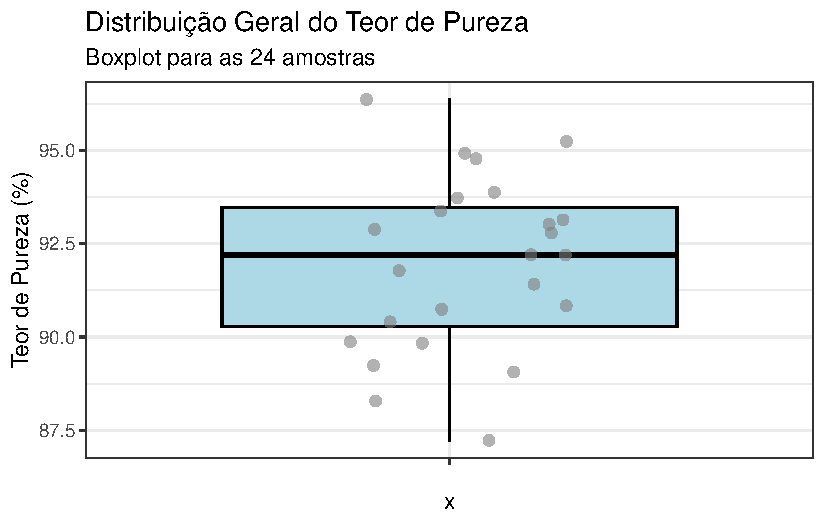
\includegraphics[keepaspectratio]{Controle_de_qualidade--3-_files/figure-pdf/unnamed-chunk-2-1.pdf}}

\begin{Shaded}
\begin{Highlighting}[]
\CommentTok{\# Carregar bibliotecas necessárias}
\FunctionTok{library}\NormalTok{(dplyr)}
\FunctionTok{library}\NormalTok{(ggplot2)}

\CommentTok{\# Calcular a diferença absoluta no teor de pureza entre amostras consecutivas}
\NormalTok{tabela\_pureza }\OtherTok{\textless{}{-}}\NormalTok{ tabela\_pureza }\SpecialCharTok{\%\textgreater{}\%}
  \FunctionTok{mutate}\NormalTok{(}\AttributeTok{Diferenca\_Pureza =} \FunctionTok{abs}\NormalTok{(Teor\_Pureza }\SpecialCharTok{{-}}\FunctionTok{mean}\NormalTok{(Teor\_Pureza)))  }\CommentTok{\# Diferença entre amostras consecutivas}

\CommentTok{\# Selecionar as 5 amostras com a maior diferença no teor de pureza}
\NormalTok{top\_5\_maior\_diferenca }\OtherTok{\textless{}{-}}\NormalTok{ tabela\_pureza }\SpecialCharTok{\%\textgreater{}\%}
  \FunctionTok{arrange}\NormalTok{(}\FunctionTok{desc}\NormalTok{(Diferenca\_Pureza)) }\SpecialCharTok{\%\textgreater{}\%}
  \FunctionTok{slice\_head}\NormalTok{(}\AttributeTok{n =} \DecValTok{5}\NormalTok{)}

\CommentTok{\# Calcular a média da diferença}
\NormalTok{media\_diferenca\_maior }\OtherTok{\textless{}{-}} \FunctionTok{mean}\NormalTok{(top\_5\_maior\_diferenca}\SpecialCharTok{$}\NormalTok{Diferenca\_Pureza, }\AttributeTok{na.rm =} \ConstantTok{TRUE}\NormalTok{)}

\CommentTok{\# Criar o gráfico de barras}
\FunctionTok{ggplot}\NormalTok{(top\_5\_maior\_diferenca, }\FunctionTok{aes}\NormalTok{(}\AttributeTok{x =} \FunctionTok{factor}\NormalTok{(Numero\_Amostra), }\AttributeTok{y =}\NormalTok{ Diferenca\_Pureza)) }\SpecialCharTok{+}
  \FunctionTok{geom\_bar}\NormalTok{(}\AttributeTok{stat =} \StringTok{"identity"}\NormalTok{, }\AttributeTok{fill =} \StringTok{"steelblue"}\NormalTok{, }\AttributeTok{color =} \StringTok{"black"}\NormalTok{) }\SpecialCharTok{+}
  \FunctionTok{geom\_hline}\NormalTok{(}\AttributeTok{yintercept =}\NormalTok{ media\_diferenca\_maior, }\AttributeTok{linetype =} \StringTok{"dashed"}\NormalTok{, }\AttributeTok{color =} \StringTok{"red"}\NormalTok{) }\SpecialCharTok{+}  \CommentTok{\# Linha de média}
  \FunctionTok{labs}\NormalTok{(}\AttributeTok{title =} \StringTok{"As 5 Amostras com Maior Diferença de Pureza"}\NormalTok{,}
       \AttributeTok{subtitle =} \StringTok{"Variação de pureza entre amostras consecutivas"}\NormalTok{,}
       \AttributeTok{x =} \StringTok{"Número da Amostra"}\NormalTok{,}
       \AttributeTok{y =} \StringTok{"Diferença Absoluta no Teor de Pureza"}\NormalTok{) }\SpecialCharTok{+}
  \FunctionTok{theme\_bw}\NormalTok{() }\SpecialCharTok{+}
  \FunctionTok{annotate}\NormalTok{(}\StringTok{"text"}\NormalTok{, }\AttributeTok{x =} \DecValTok{3}\NormalTok{, }\AttributeTok{y =}\NormalTok{ media\_diferenca\_maior }\SpecialCharTok{+} \FloatTok{0.1}\NormalTok{, }\AttributeTok{label =} \FunctionTok{paste}\NormalTok{(}\StringTok{"Média ="}\NormalTok{, }\FunctionTok{round}\NormalTok{(media\_diferenca\_maior, }\DecValTok{2}\NormalTok{)), }\AttributeTok{color =} \StringTok{"red"}\NormalTok{)}
\end{Highlighting}
\end{Shaded}

\pandocbounded{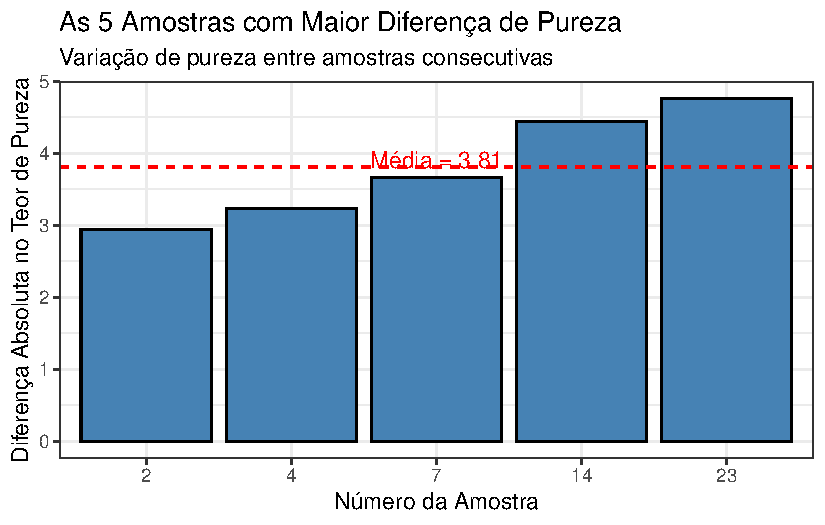
\includegraphics[keepaspectratio]{Controle_de_qualidade--3-_files/figure-pdf/unnamed-chunk-3-1.pdf}}

\begin{Shaded}
\begin{Highlighting}[]
\CommentTok{\# Calcular a diferença absoluta no teor de pureza entre amostras consecutivas}
\NormalTok{tabela\_pureza }\OtherTok{\textless{}{-}}\NormalTok{ tabela\_pureza }\SpecialCharTok{\%\textgreater{}\%}
  \FunctionTok{mutate}\NormalTok{(}\AttributeTok{Diferenca\_Pureza =} \FunctionTok{abs}\NormalTok{(Teor\_Pureza }\SpecialCharTok{{-}} \FunctionTok{mean}\NormalTok{(Teor\_Pureza)))  }\CommentTok{\# Diferença entre amostras consecutivas}

\CommentTok{\# Selecionar as 5 amostras com a menor diferença no teor de pureza}
\NormalTok{top\_5\_menor\_diferenca }\OtherTok{\textless{}{-}}\NormalTok{ tabela\_pureza }\SpecialCharTok{\%\textgreater{}\%}
  \FunctionTok{arrange}\NormalTok{(Diferenca\_Pureza) }\SpecialCharTok{\%\textgreater{}\%}
  \FunctionTok{slice\_head}\NormalTok{(}\AttributeTok{n =} \DecValTok{5}\NormalTok{)}

\CommentTok{\# Calcular a média da diferença}
\NormalTok{media\_diferenca }\OtherTok{\textless{}{-}} \FunctionTok{mean}\NormalTok{(top\_5\_menor\_diferenca}\SpecialCharTok{$}\NormalTok{Diferenca\_Pureza, }\AttributeTok{na.rm =} \ConstantTok{TRUE}\NormalTok{)}

\CommentTok{\# Criar o gráfico de barras}
\FunctionTok{ggplot}\NormalTok{(top\_5\_menor\_diferenca, }\FunctionTok{aes}\NormalTok{(}\AttributeTok{x =} \FunctionTok{factor}\NormalTok{(Numero\_Amostra), }\AttributeTok{y =}\NormalTok{ Diferenca\_Pureza)) }\SpecialCharTok{+}
  \FunctionTok{geom\_bar}\NormalTok{(}\AttributeTok{stat =} \StringTok{"identity"}\NormalTok{, }\AttributeTok{fill =} \StringTok{"orange"}\NormalTok{, }\AttributeTok{color =} \StringTok{"black"}\NormalTok{) }\SpecialCharTok{+}
  \FunctionTok{geom\_hline}\NormalTok{(}\AttributeTok{yintercept =}\NormalTok{ media\_diferenca, }\AttributeTok{linetype =} \StringTok{"dashed"}\NormalTok{, }\AttributeTok{color =} \StringTok{"red"}\NormalTok{) }\SpecialCharTok{+}  \CommentTok{\# Linha de média}
  \FunctionTok{labs}\NormalTok{(}\AttributeTok{title =} \StringTok{"As 5 Amostras com Menor Diferença de Pureza"}\NormalTok{,}
       \AttributeTok{subtitle =} \StringTok{"Variação de pureza entre amostras consecutivas"}\NormalTok{,}
       \AttributeTok{x =} \StringTok{"Número da Amostra"}\NormalTok{,}
       \AttributeTok{y =} \StringTok{"Diferença Absoluta no Teor de Pureza"}\NormalTok{) }\SpecialCharTok{+}
  \FunctionTok{theme\_bw}\NormalTok{() }\SpecialCharTok{+}
  \FunctionTok{annotate}\NormalTok{(}\StringTok{"text"}\NormalTok{, }\AttributeTok{x =} \DecValTok{3}\NormalTok{, }\AttributeTok{y =}\NormalTok{ media\_diferenca }\SpecialCharTok{+} \FloatTok{0.1}\NormalTok{, }\AttributeTok{label =} \FunctionTok{paste}\NormalTok{(}\StringTok{"Média ="}\NormalTok{, }\FunctionTok{round}\NormalTok{(media\_diferenca, }\DecValTok{2}\NormalTok{)), }\AttributeTok{color =} \StringTok{"red"}\NormalTok{)}
\end{Highlighting}
\end{Shaded}

\pandocbounded{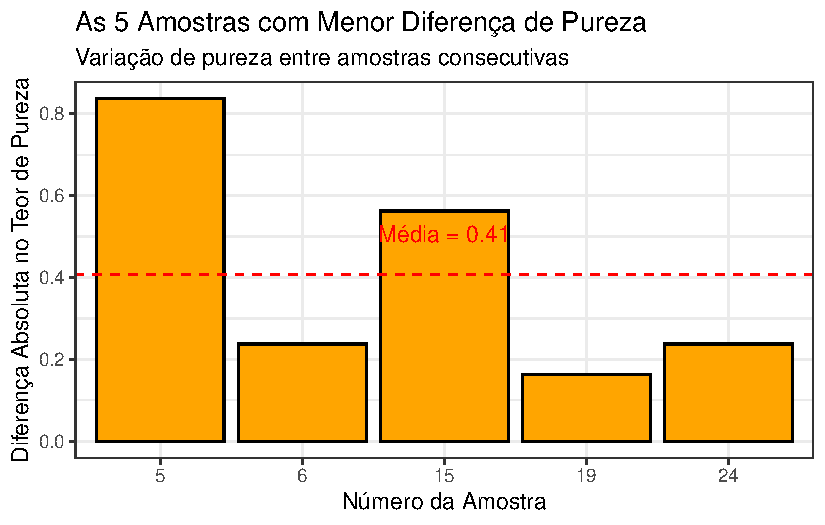
\includegraphics[keepaspectratio]{Controle_de_qualidade--3-_files/figure-pdf/unnamed-chunk-4-1.pdf}}

\subsubsection{Calculando as médias}\label{calculando-as-muxe9dias}

\begin{Shaded}
\begin{Highlighting}[]
\NormalTok{X\_bar }\OtherTok{\textless{}{-}} \FunctionTok{mean}\NormalTok{(tabela\_pureza}\SpecialCharTok{$}\NormalTok{Teor\_Pureza)}
\NormalTok{AM\_bar }\OtherTok{\textless{}{-}} \FunctionTok{mean}\NormalTok{(}\FunctionTok{na.omit}\NormalTok{(tabela\_pureza}\SpecialCharTok{$}\NormalTok{Amplitude\_Movel))}
\CommentTok{\# Exibindo os valores médios}
\FunctionTok{cat}\NormalTok{(}\StringTok{"Média do Teor de Pureza:"}\NormalTok{, X\_bar, }\StringTok{"}\SpecialCharTok{\textbackslash{}n}\StringTok{"}\NormalTok{)}
\end{Highlighting}
\end{Shaded}

\begin{verbatim}
Média do Teor de Pureza: 91.9625 
\end{verbatim}

\begin{Shaded}
\begin{Highlighting}[]
\FunctionTok{cat}\NormalTok{(}\StringTok{"Média da Amplitude Móvel:"}\NormalTok{, AM\_bar, }\StringTok{"}\SpecialCharTok{\textbackslash{}n}\StringTok{"}\NormalTok{)}
\end{Highlighting}
\end{Shaded}

\begin{verbatim}
Média da Amplitude Móvel: 2.821739 
\end{verbatim}

\subsubsection{Resumo geral}\label{resumo-geral}

\begin{Shaded}
\begin{Highlighting}[]
\CommentTok{\# Calcular o resumo estatístico para a coluna "Teor\_Pureza" e "Amplitude\_Movel"}
\NormalTok{resumo }\OtherTok{\textless{}{-}} \FunctionTok{summary}\NormalTok{(}\FunctionTok{na.omit}\NormalTok{(tabela\_pureza[, }\FunctionTok{c}\NormalTok{(}\DecValTok{2}\NormalTok{, }\DecValTok{3}\NormalTok{)])); resumo}
\end{Highlighting}
\end{Shaded}

\begin{verbatim}
  Teor_Pureza    Amplitude_Movel
 Min.   :87.20   Min.   :0.600  
 1st Qu.:90.15   1st Qu.:1.450  
 Median :92.20   Median :2.300  
 Mean   :91.92   Mean   :2.822  
 3rd Qu.:93.55   3rd Qu.:4.200  
 Max.   :96.40   Max.   :6.200  
\end{verbatim}

\subsubsection{Cálculo dos limites de controle para os gráfico X e
AM}\label{cuxe1lculo-dos-limites-de-controle-para-os-gruxe1fico-x-e-am}

\begin{Shaded}
\begin{Highlighting}[]
\NormalTok{X\_bar }\OtherTok{=} \FunctionTok{mean}\NormalTok{(Teor\_Pureza)}
\NormalTok{AM\_bar }\OtherTok{=} \FunctionTok{mean}\NormalTok{(}\FunctionTok{na.omit}\NormalTok{(Amplitude\_Movel))}

\NormalTok{D3 }\OtherTok{=} \DecValTok{0}\NormalTok{ ; D4 }\OtherTok{=} \FloatTok{3.267}\NormalTok{ ; d2 }\OtherTok{=} \FloatTok{1.128}
  
\CommentTok{\# Cálculo dos limites de controle para os gráfico AM}
\NormalTok{LSC\_X }\OtherTok{\textless{}{-}}\NormalTok{ X\_bar }\SpecialCharTok{+} \DecValTok{3}\SpecialCharTok{*}\NormalTok{(AM\_bar}\SpecialCharTok{/}\NormalTok{d2);}
\NormalTok{LM }\OtherTok{=}\NormalTok{ X\_bar;}
\NormalTok{LIC\_X }\OtherTok{\textless{}{-}}\NormalTok{ X\_bar }\SpecialCharTok{{-}} \DecValTok{3}\SpecialCharTok{*}\NormalTok{(AM\_bar}\SpecialCharTok{/}\NormalTok{d2);}

\CommentTok{\# Cálculo dos limites de controle para os gráfico X}
\NormalTok{LSC\_AM }\OtherTok{\textless{}{-}}\NormalTok{D4}\SpecialCharTok{*}\NormalTok{AM\_bar;}
\NormalTok{LM }\OtherTok{=}\NormalTok{ AM\_bar;}
\NormalTok{LIC\_AM }\OtherTok{\textless{}{-}}\NormalTok{D3}\SpecialCharTok{*}\NormalTok{AM\_bar;}

\CommentTok{\# Exibir os limites calculados}
\FunctionTok{cat}\NormalTok{(}\StringTok{"Limites de Controle para o Gráfico expression(AM):}\SpecialCharTok{\textbackslash{}n}\StringTok{"}\NormalTok{)}
\end{Highlighting}
\end{Shaded}

\begin{verbatim}
Limites de Controle para o Gráfico expression(AM):
\end{verbatim}

\begin{Shaded}
\begin{Highlighting}[]
\FunctionTok{cat}\NormalTok{(}\StringTok{"LSC:"}\NormalTok{, LSC\_AM, }\StringTok{"}\SpecialCharTok{\textbackslash{}n}\StringTok{"}\NormalTok{)}
\end{Highlighting}
\end{Shaded}

\begin{verbatim}
LSC: 9.218622 
\end{verbatim}

\begin{Shaded}
\begin{Highlighting}[]
\FunctionTok{cat}\NormalTok{(}\StringTok{"LIC:"}\NormalTok{, LIC\_AM, }\StringTok{"}\SpecialCharTok{\textbackslash{}n\textbackslash{}n}\StringTok{"}\NormalTok{)}
\end{Highlighting}
\end{Shaded}

\begin{verbatim}
LIC: 0 
\end{verbatim}

\begin{Shaded}
\begin{Highlighting}[]
\FunctionTok{cat}\NormalTok{(}\StringTok{"Limites de Controle para o Gráfico X:}\SpecialCharTok{\textbackslash{}n}\StringTok{"}\NormalTok{)}
\end{Highlighting}
\end{Shaded}

\begin{verbatim}
Limites de Controle para o Gráfico X:
\end{verbatim}

\begin{Shaded}
\begin{Highlighting}[]
\FunctionTok{cat}\NormalTok{(}\StringTok{"LSC:"}\NormalTok{, LSC\_X, }\StringTok{"}\SpecialCharTok{\textbackslash{}n}\StringTok{"}\NormalTok{)}
\end{Highlighting}
\end{Shaded}

\begin{verbatim}
LSC: 99.46713 
\end{verbatim}

\begin{Shaded}
\begin{Highlighting}[]
\FunctionTok{cat}\NormalTok{(}\StringTok{"LIC:"}\NormalTok{, LIC\_X, }\StringTok{"}\SpecialCharTok{\textbackslash{}n}\StringTok{"}\NormalTok{)}
\end{Highlighting}
\end{Shaded}

\begin{verbatim}
LIC: 84.45787 
\end{verbatim}

\subsubsection{Gráfico para Medidas
Individuais}\label{gruxe1fico-para-medidas-individuais}

\subsubsection{O Limite Médio (LM) é obtido a partir da média geral das
amostras. Para calcular os Limites de Controle da média, utiliza-se a
constante
d2.}\label{o-limite-muxe9dio-lm-uxe9-obtido-a-partir-da-muxe9dia-geral-das-amostras.-para-calcular-os-limites-de-controle-da-muxe9dia-utiliza-se-a-constante-d2.}

\begin{Shaded}
\begin{Highlighting}[]
\CommentTok{\# Cálculo das médias e desvios padrão das amostras}
\CommentTok{\# vetor\_medias \textless{}{-} rowMeans(Teor\_Pureza)}
\CommentTok{\# vetor\_desvios \textless{}{-} apply(dados, 1, sd)}
\CommentTok{\# }
\CommentTok{\# dados$medias \textless{}{-} vetor\_medias}
\CommentTok{\# dados$desvios \textless{}{-} vetor\_desvios}

\CommentTok{\# Gráfico de Controle X̄ interativo}
\NormalTok{grafico\_X }\OtherTok{\textless{}{-}} \FunctionTok{plot\_ly}\NormalTok{(}\AttributeTok{x =} \FunctionTok{seq\_along}\NormalTok{(Teor\_Pureza), }\AttributeTok{y =}\NormalTok{ Teor\_Pureza, }\AttributeTok{type =} \StringTok{\textquotesingle{}scatter\textquotesingle{}}\NormalTok{, }\AttributeTok{mode =} \StringTok{\textquotesingle{}lines+markers\textquotesingle{}}\NormalTok{,}
                     \AttributeTok{name =} \StringTok{\textquotesingle{}Média das Amostras\textquotesingle{}}\NormalTok{) }\SpecialCharTok{\%\textgreater{}\%}
  \FunctionTok{add\_trace}\NormalTok{(}\AttributeTok{y =} \FunctionTok{rep}\NormalTok{(X\_bar, }\FunctionTok{length}\NormalTok{(Teor\_Pureza)), }\AttributeTok{mode =} \StringTok{"lines"}\NormalTok{, }\AttributeTok{name =} \StringTok{"Média X̄"}\NormalTok{, }\AttributeTok{line =} \FunctionTok{list}\NormalTok{(}\AttributeTok{color =} \StringTok{"blue"}\NormalTok{)) }\SpecialCharTok{\%\textgreater{}\%}
  \FunctionTok{add\_trace}\NormalTok{(}\AttributeTok{y =} \FunctionTok{rep}\NormalTok{(LSC\_X, }\FunctionTok{length}\NormalTok{(Teor\_Pureza)), }\AttributeTok{mode =} \StringTok{"lines"}\NormalTok{, }\AttributeTok{name =} \StringTok{"LSC"}\NormalTok{, }\AttributeTok{line =} \FunctionTok{list}\NormalTok{(}\AttributeTok{color =} \StringTok{"red"}\NormalTok{, }\AttributeTok{dash =} \StringTok{\textquotesingle{}dash\textquotesingle{}}\NormalTok{)) }\SpecialCharTok{\%\textgreater{}\%}
  \FunctionTok{add\_trace}\NormalTok{(}\AttributeTok{y =} \FunctionTok{rep}\NormalTok{(LIC\_X, }\FunctionTok{length}\NormalTok{(Teor\_Pureza)), }\AttributeTok{mode =} \StringTok{"lines"}\NormalTok{, }\AttributeTok{name =} \StringTok{"LIC"}\NormalTok{, }\AttributeTok{line =} \FunctionTok{list}\NormalTok{(}\AttributeTok{color =} \StringTok{"red"}\NormalTok{, }\AttributeTok{dash =} \StringTok{\textquotesingle{}dash\textquotesingle{}}\NormalTok{)) }\SpecialCharTok{\%\textgreater{}\%}
  \FunctionTok{layout}\NormalTok{(}\AttributeTok{title =} \StringTok{"Gráfico de Controle X̄"}\NormalTok{,}
         \AttributeTok{xaxis =} \FunctionTok{list}\NormalTok{(}\AttributeTok{title =} \StringTok{"Amostra"}\NormalTok{),}
         \AttributeTok{yaxis =} \FunctionTok{list}\NormalTok{(}\AttributeTok{title =} \StringTok{"Média"}\NormalTok{))}
\NormalTok{grafico\_X}
\end{Highlighting}
\end{Shaded}

\begin{verbatim}
file:///C:/Users/fabia/AppData/Local/Temp/Rtmp4KpvhV/file2b146cf2b35/widget2b145742ed5.html screenshot completed
\end{verbatim}

\pandocbounded{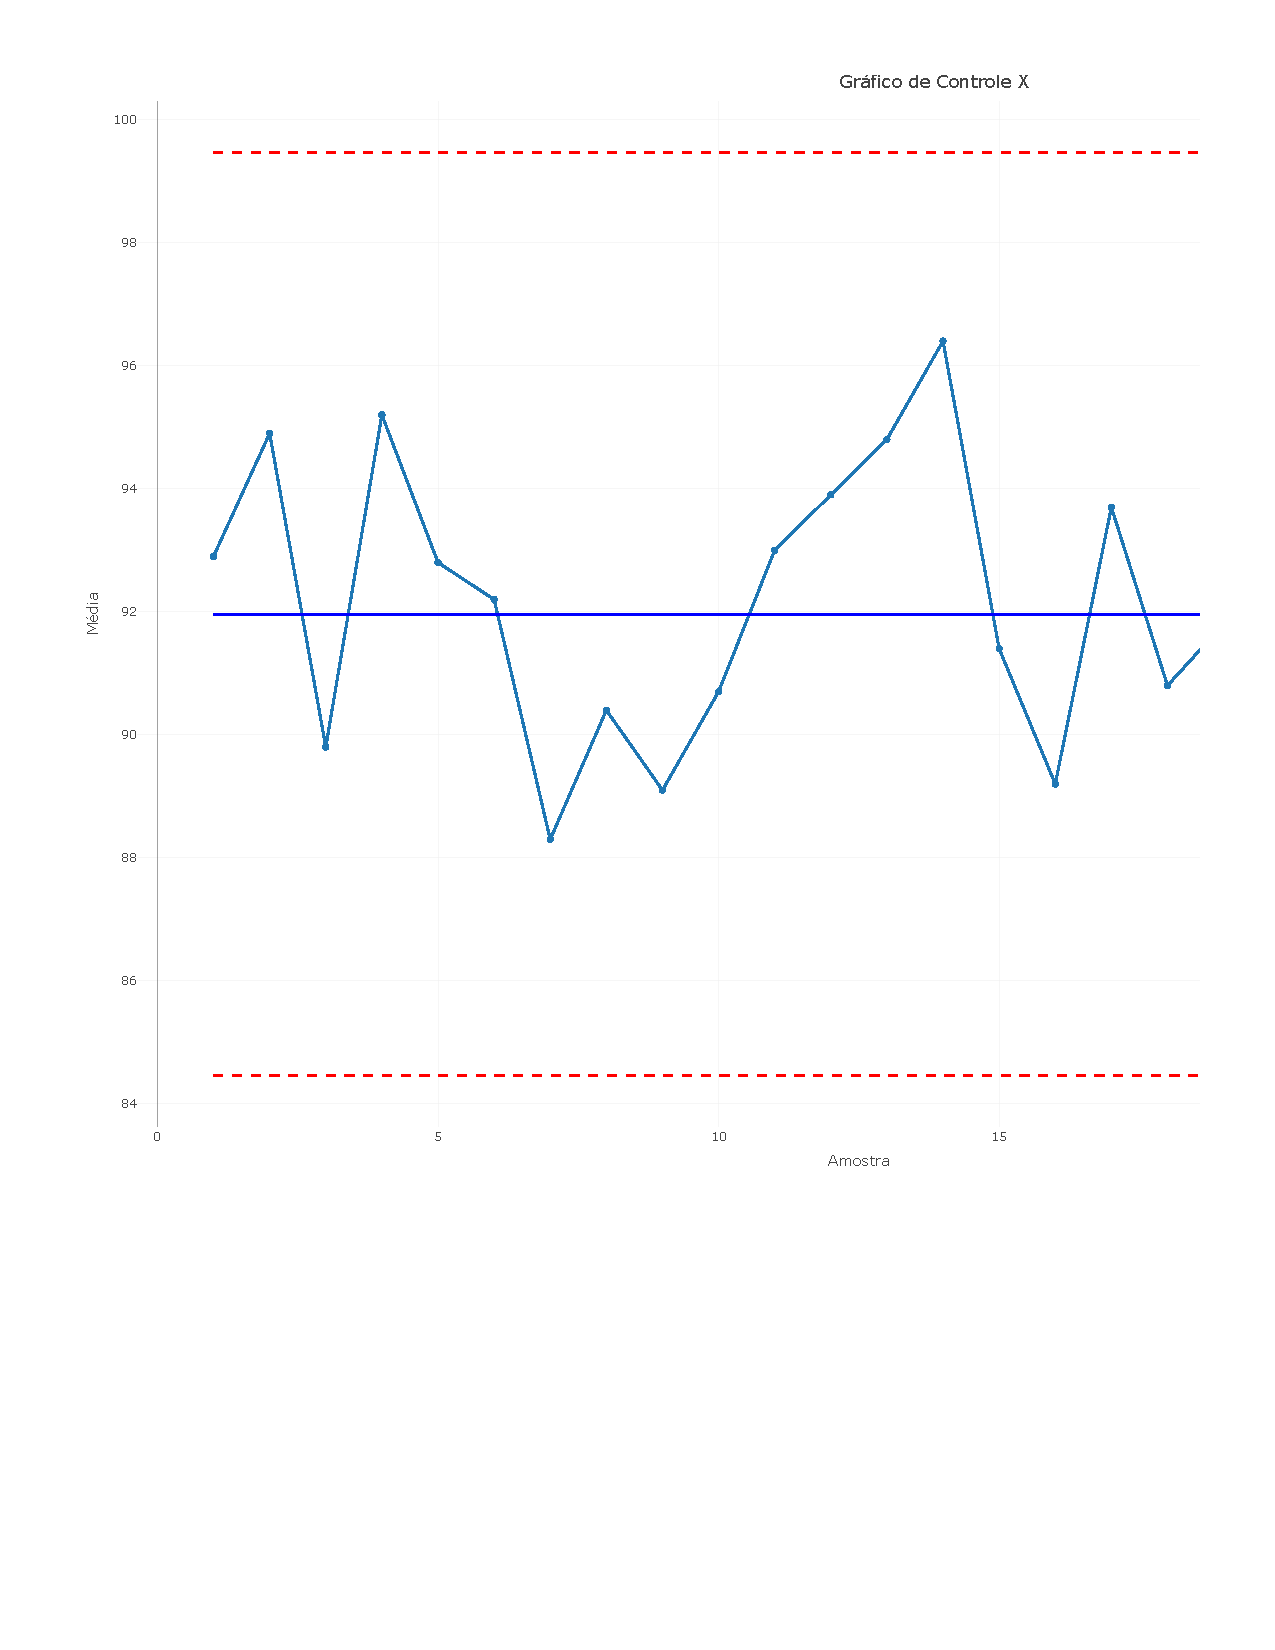
\includegraphics[keepaspectratio]{Controle_de_qualidade--3-_files/figure-pdf/unnamed-chunk-8-1.pdf}}

\subsubsection{Gráfico para a amplitude
móvel}\label{gruxe1fico-para-a-amplitude-muxf3vel}

\subsubsection{Nesta fase, iniciamos o cálculo dos limites de controle
inferior (LIC) e superior (LSC). Para determinar esses limites, é
necessário calcular a amplitude média das amostras. Para o cálculo do
Limite Inferior de Controle (LIC), utilizamos a constante D3, enquanto
para o Limite Superior de Controle (LSC), aplicamos a constante
D4.}\label{nesta-fase-iniciamos-o-cuxe1lculo-dos-limites-de-controle-inferior-lic-e-superior-lsc.-para-determinar-esses-limites-uxe9-necessuxe1rio-calcular-a-amplitude-muxe9dia-das-amostras.-para-o-cuxe1lculo-do-limite-inferior-de-controle-lic-utilizamos-a-constante-d3-enquanto-para-o-limite-superior-de-controle-lsc-aplicamos-a-constante-d4.}

\begin{Shaded}
\begin{Highlighting}[]
\CommentTok{\# Gráfico de Controle AM interativo}
\NormalTok{grafico\_AM }\OtherTok{\textless{}{-}} \FunctionTok{plot\_ly}\NormalTok{(}\AttributeTok{x =} \FunctionTok{seq\_along}\NormalTok{(Amplitude\_Movel), }\AttributeTok{y =}\NormalTok{ Amplitude\_Movel, }\AttributeTok{type =} \StringTok{\textquotesingle{}scatter\textquotesingle{}}\NormalTok{, }\AttributeTok{mode =} \StringTok{\textquotesingle{}lines+markers\textquotesingle{}}\NormalTok{,}
                     \AttributeTok{name =} \StringTok{\textquotesingle{}Desvio Padrão\textquotesingle{}}\NormalTok{) }\SpecialCharTok{\%\textgreater{}\%}
  \FunctionTok{add\_trace}\NormalTok{(}\AttributeTok{y =} \FunctionTok{rep}\NormalTok{(AM\_bar, }\FunctionTok{length}\NormalTok{(Amplitude\_Movel)), }\AttributeTok{mode =} \StringTok{"lines"}\NormalTok{, }\AttributeTok{name =} \StringTok{"Média AM"}\NormalTok{, }\AttributeTok{line =} \FunctionTok{list}\NormalTok{(}\AttributeTok{color =} \StringTok{"blue"}\NormalTok{)) }\SpecialCharTok{\%\textgreater{}\%}
  \FunctionTok{add\_trace}\NormalTok{(}\AttributeTok{y =} \FunctionTok{rep}\NormalTok{(LSC\_AM, }\FunctionTok{length}\NormalTok{(Amplitude\_Movel)), }\AttributeTok{mode =} \StringTok{"lines"}\NormalTok{, }\AttributeTok{name =} \StringTok{"LSC"}\NormalTok{, }\AttributeTok{line =} \FunctionTok{list}\NormalTok{(}\AttributeTok{color =} \StringTok{"red"}\NormalTok{, }\AttributeTok{dash =} \StringTok{\textquotesingle{}dash\textquotesingle{}}\NormalTok{)) }\SpecialCharTok{\%\textgreater{}\%}
  \FunctionTok{add\_trace}\NormalTok{(}\AttributeTok{y =} \FunctionTok{rep}\NormalTok{(LIC\_AM, }\FunctionTok{length}\NormalTok{(Amplitude\_Movel)), }\AttributeTok{mode =} \StringTok{"lines"}\NormalTok{, }\AttributeTok{name =} \StringTok{"LIC"}\NormalTok{, }\AttributeTok{line =} \FunctionTok{list}\NormalTok{(}\AttributeTok{color =} \StringTok{"red"}\NormalTok{, }\AttributeTok{dash =} \StringTok{\textquotesingle{}dash\textquotesingle{}}\NormalTok{)) }\SpecialCharTok{\%\textgreater{}\%}
  \FunctionTok{layout}\NormalTok{(}\AttributeTok{title =} \StringTok{"Gráfico de Controle AM"}\NormalTok{,}
         \AttributeTok{xaxis =} \FunctionTok{list}\NormalTok{(}\AttributeTok{title =} \StringTok{"Amostra"}\NormalTok{),}
         \AttributeTok{yaxis =} \FunctionTok{list}\NormalTok{(}\AttributeTok{title =} \StringTok{"Desvio Padrão"}\NormalTok{))}

\CommentTok{\# Exibir os gráficos interativos}
\NormalTok{grafico\_AM}
\end{Highlighting}
\end{Shaded}

\begin{verbatim}
file:///C:/Users/fabia/AppData/Local/Temp/Rtmp4KpvhV/file2b146ba3598/widget2b1411432e60.html screenshot completed
\end{verbatim}

\pandocbounded{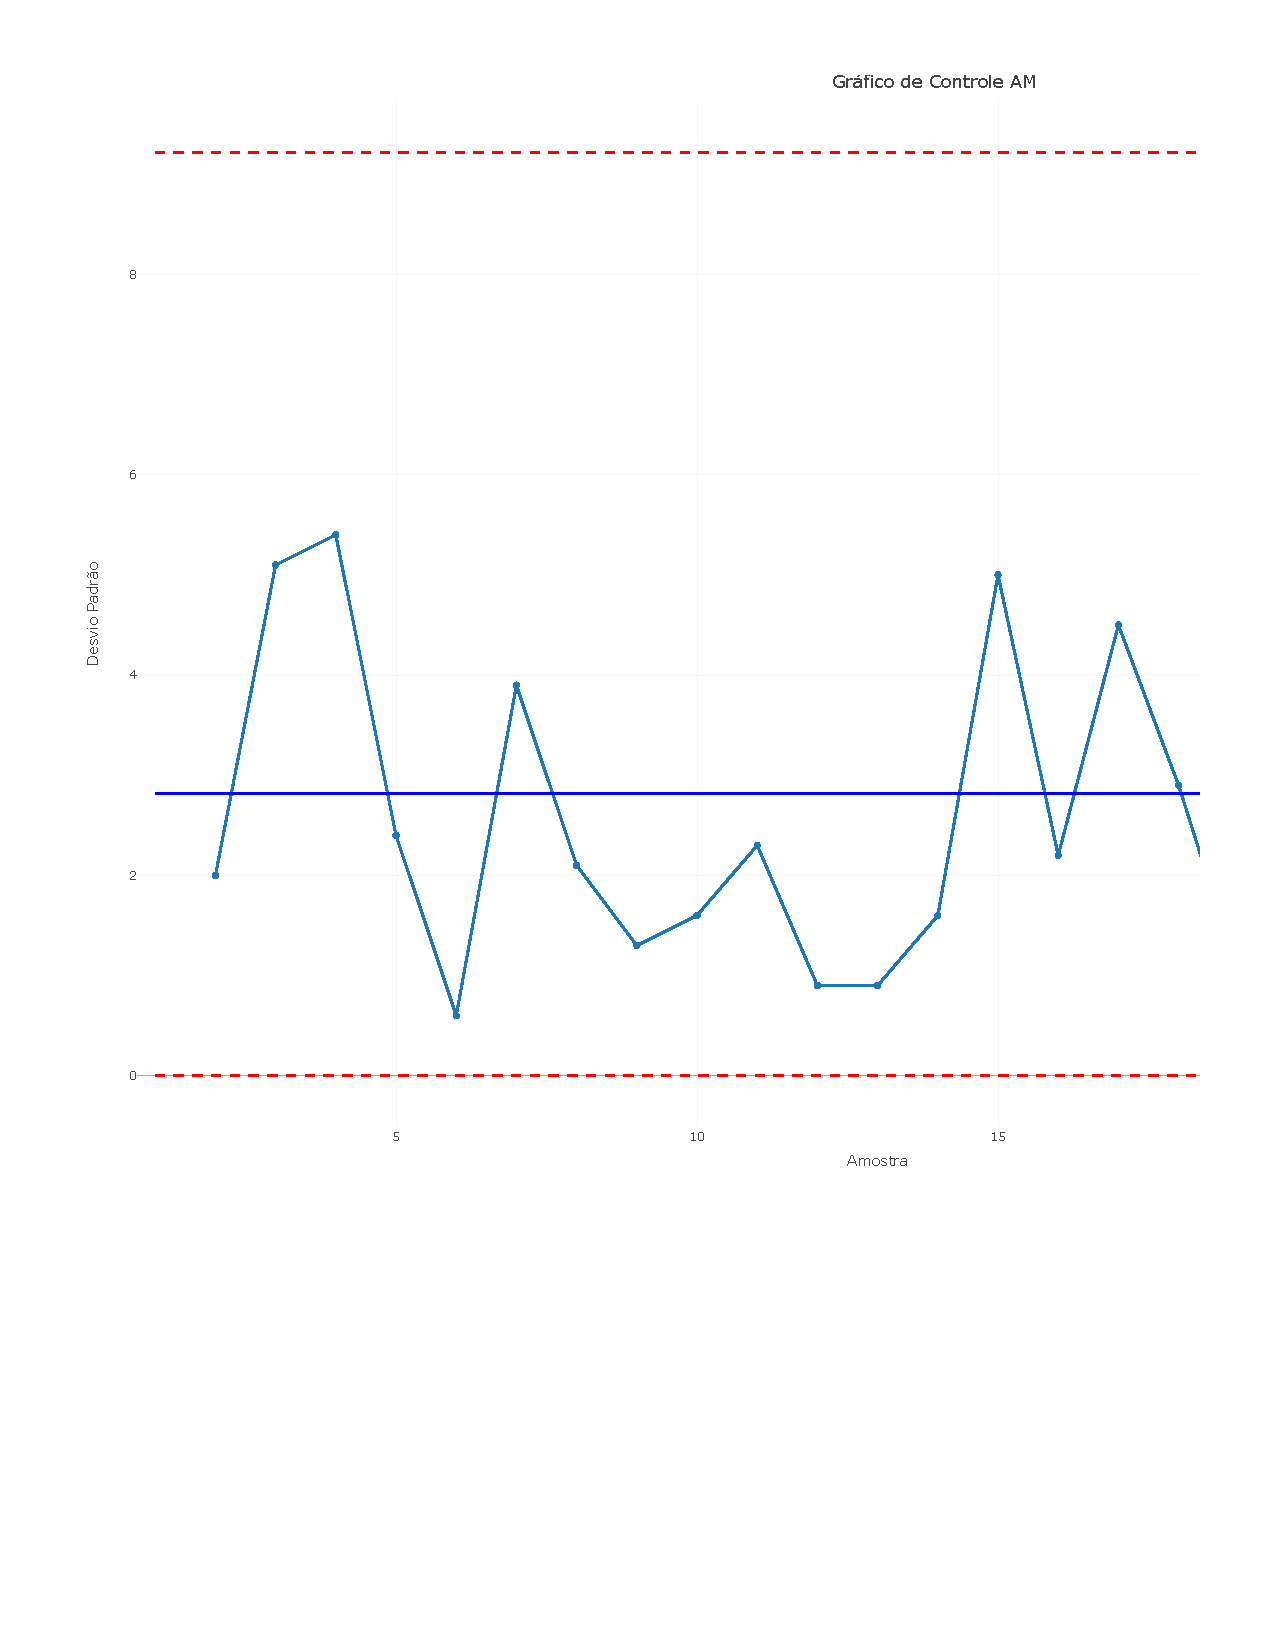
\includegraphics[keepaspectratio]{Controle_de_qualidade--3-_files/figure-pdf/unnamed-chunk-9-1.pdf}}

\subsubsection{Nenhuma amostra fora de controle foi identificada no
gráfico de medidas Individuais, isso indica a ausência de amostras fora
de controle no gráfico de medidas individuais indica que o processo está
estável e dentro dos limites esperados, sem variações
especiais.}\label{nenhuma-amostra-fora-de-controle-foi-identificada-no-gruxe1fico-de-medidas-individuais-isso-indica-a-ausuxeancia-de-amostras-fora-de-controle-no-gruxe1fico-de-medidas-individuais-indica-que-o-processo-estuxe1-estuxe1vel-e-dentro-dos-limites-esperados-sem-variauxe7uxf5es-especiais.}

\subsubsection{Análise Estatística das 48
amostras:}\label{anuxe1lise-estatuxedstica-das-48-amostras}

\begin{Shaded}
\begin{Highlighting}[]
\CommentTok{\# Para as 23 amotras de }
\NormalTok{tabela\_pureza2 }\OtherTok{\textless{}{-}} \FunctionTok{data.frame}\NormalTok{(}
  \AttributeTok{Numero\_Amostra1 =} \DecValTok{1}\SpecialCharTok{:}\DecValTok{48}\NormalTok{,}
  \AttributeTok{Teor\_Pureza1 =} \FunctionTok{c}\NormalTok{(}\FloatTok{92.9}\NormalTok{, }\FloatTok{94.9}\NormalTok{, }\FloatTok{89.8}\NormalTok{, }\FloatTok{95.2}\NormalTok{, }\FloatTok{92.8}\NormalTok{, }\FloatTok{92.2}\NormalTok{, }\FloatTok{88.3}\NormalTok{, }\FloatTok{90.4}\NormalTok{, }\FloatTok{89.1}\NormalTok{, }\FloatTok{90.7}\NormalTok{, }
                  \FloatTok{93.0}\NormalTok{, }\FloatTok{93.9}\NormalTok{, }\FloatTok{94.8}\NormalTok{, }\FloatTok{96.4}\NormalTok{, }\FloatTok{91.4}\NormalTok{, }\FloatTok{89.2}\NormalTok{, }\FloatTok{93.7}\NormalTok{, }\FloatTok{90.8}\NormalTok{, }\FloatTok{91.8}\NormalTok{, }\FloatTok{93.1}\NormalTok{, }
                  \FloatTok{89.9}\NormalTok{, }\FloatTok{93.4}\NormalTok{, }\FloatTok{87.2}\NormalTok{, }\FloatTok{92.2}\NormalTok{,}\FloatTok{93.2}\NormalTok{,}\FloatTok{94.9}\NormalTok{,}\FloatTok{89.7}\NormalTok{,}\FloatTok{95.8}\NormalTok{,}\FloatTok{92.6}\NormalTok{,}\FloatTok{92.2}\NormalTok{,}\FloatTok{80.1}\NormalTok{,}
                  \FloatTok{82.7}\NormalTok{,}\DecValTok{81}\NormalTok{,}\FloatTok{82.7}\NormalTok{,}\FloatTok{85.3}\NormalTok{,}\FloatTok{85.9}\NormalTok{,}\FloatTok{86.8}\NormalTok{,}\FloatTok{86.3}\NormalTok{,}\FloatTok{83.7}\NormalTok{,}\FloatTok{81.5}\NormalTok{,}\FloatTok{86.9}\NormalTok{,}\FloatTok{82.7}\NormalTok{,}\DecValTok{84}\NormalTok{,}
                  \FloatTok{85.2}\NormalTok{,}\FloatTok{82.8}\NormalTok{,}\DecValTok{85}\NormalTok{,}\FloatTok{87.2}\NormalTok{,}\FloatTok{82.6}\NormalTok{),}
  \AttributeTok{Amplitude\_Movel1 =} \FunctionTok{c}\NormalTok{(}\ConstantTok{NA}\NormalTok{, }\FloatTok{2.0}\NormalTok{, }\FloatTok{5.1}\NormalTok{, }\FloatTok{5.4}\NormalTok{, }\FloatTok{2.4}\NormalTok{, }\FloatTok{0.6}\NormalTok{, }\FloatTok{3.9}\NormalTok{, }\FloatTok{2.1}\NormalTok{, }\FloatTok{1.3}\NormalTok{, }\FloatTok{1.6}\NormalTok{, }
                      \FloatTok{2.3}\NormalTok{, }\FloatTok{0.9}\NormalTok{, }\FloatTok{0.9}\NormalTok{, }\FloatTok{1.6}\NormalTok{, }\FloatTok{5.0}\NormalTok{, }\FloatTok{2.2}\NormalTok{, }\FloatTok{4.5}\NormalTok{, }\FloatTok{2.9}\NormalTok{, }\FloatTok{1.0}\NormalTok{, }\FloatTok{1.3}\NormalTok{, }
                      \FloatTok{3.2}\NormalTok{, }\FloatTok{3.5}\NormalTok{, }\FloatTok{6.2}\NormalTok{, }\FloatTok{5.0}\NormalTok{,}\FloatTok{1.0}\NormalTok{,}\FloatTok{1.7}\NormalTok{,}\FloatTok{5.2}\NormalTok{,}\FloatTok{6.1}\NormalTok{,}\FloatTok{3.2}\NormalTok{,}\FloatTok{0.4}\NormalTok{,}\FloatTok{12.2}\NormalTok{,}\FloatTok{2.6}\NormalTok{,}
                      \FloatTok{1.7}\NormalTok{,}\FloatTok{1.7}\NormalTok{,}\FloatTok{2.6}\NormalTok{,}\FloatTok{0.6}\NormalTok{,}\FloatTok{0.9}\NormalTok{,}\FloatTok{0.5}\NormalTok{,}\FloatTok{2.6}\NormalTok{,}\FloatTok{2.2}\NormalTok{,}\FloatTok{5.4}\NormalTok{,}\FloatTok{4.2}\NormalTok{,}\FloatTok{1.3}\NormalTok{,}\FloatTok{1.2}\NormalTok{,}\FloatTok{2.4}\NormalTok{,}\FloatTok{2.2}\NormalTok{,}
                      \FloatTok{2.2}\NormalTok{,}\FloatTok{4.6}\NormalTok{)}
\NormalTok{)}
\end{Highlighting}
\end{Shaded}

\subsubsection{Análise descritiva}\label{anuxe1lise-descritiva-1}

\subsubsection{Boxplot para estudar a diferenças entre os Teor de pureza
das 48 amostras estudadas para o Teour de
Pureza}\label{boxplot-para-estudar-a-diferenuxe7as-entre-os-teor-de-pureza-das-48-amostras-estudadas-para-o-teour-de-pureza}

\begin{Shaded}
\begin{Highlighting}[]
\FunctionTok{library}\NormalTok{(dplyr)}
\FunctionTok{library}\NormalTok{(ggplot2)}

\CommentTok{\# Criar uma coluna categórica para identificar os pontos fora dos limites}
\NormalTok{tabela\_pureza2 }\OtherTok{\textless{}{-}}\NormalTok{ tabela\_pureza2 }\SpecialCharTok{\%\textgreater{}\%}
  \FunctionTok{mutate}\NormalTok{(}\AttributeTok{Classificacao2 =} \FunctionTok{case\_when}\NormalTok{(}
\NormalTok{    Teor\_Pureza1 }\SpecialCharTok{\textgreater{}} \FunctionTok{mean}\NormalTok{(Teor\_Pureza1) }\SpecialCharTok{\textasciitilde{}} \StringTok{"Acima da média "}\NormalTok{,}
\NormalTok{    Teor\_Pureza1 }\SpecialCharTok{\textless{}} \FunctionTok{mean}\NormalTok{(Teor\_Pureza1) }\SpecialCharTok{\textasciitilde{}} \StringTok{"Abaixo da média"}\NormalTok{,}
    \ConstantTok{TRUE} \SpecialCharTok{\textasciitilde{}} \StringTok{"Dentro dos Limites"}  \CommentTok{\# Condição padrão}
\NormalTok{  ))}

\CommentTok{\# Criar o boxplot com os pontos coloridos por categoria}
\FunctionTok{ggplot}\NormalTok{(tabela\_pureza2, }\FunctionTok{aes}\NormalTok{(}\AttributeTok{x =} \StringTok{""}\NormalTok{, }\AttributeTok{y =}\NormalTok{ Teor\_Pureza1)) }\SpecialCharTok{+}
  \FunctionTok{geom\_boxplot}\NormalTok{(}\AttributeTok{fill =} \StringTok{"lightblue"}\NormalTok{, }\AttributeTok{color =} \StringTok{"black"}\NormalTok{) }\SpecialCharTok{+}
  \FunctionTok{geom\_jitter}\NormalTok{(}\FunctionTok{aes}\NormalTok{(}\AttributeTok{color =}\NormalTok{ Classificacao2), }\AttributeTok{width =} \FloatTok{0.2}\NormalTok{, }\AttributeTok{size =} \DecValTok{2}\NormalTok{, }\AttributeTok{alpha =} \FloatTok{0.6}\NormalTok{) }\SpecialCharTok{+}
  \FunctionTok{scale\_color\_manual}\NormalTok{(}
    \AttributeTok{name =} \StringTok{"Status da amostra"}\NormalTok{,  }\CommentTok{\# Novo título da legenda}
    \AttributeTok{values =} \FunctionTok{c}\NormalTok{(}\StringTok{"Abaixo do LIC"} \OtherTok{=} \StringTok{"blue"}\NormalTok{,  }\StringTok{"Dentro dos Limites"} \OtherTok{=} \StringTok{"green"}\NormalTok{, }\StringTok{"Acima do LSC"} \OtherTok{=} \StringTok{"red"}\NormalTok{),}
    \AttributeTok{labels =} \FunctionTok{c}\NormalTok{(}\StringTok{"Abaixo do limite de qualidade"}\NormalTok{,}\StringTok{"Dentro do padrão de qualidade"}\NormalTok{,}\StringTok{"Acima do limite de qualidade"}\NormalTok{)}
\NormalTok{  ) }\SpecialCharTok{+}
  \FunctionTok{labs}\NormalTok{(}\AttributeTok{title =} \StringTok{"Distribuição Geral do Teor de Pureza"}\NormalTok{,}
       \AttributeTok{subtitle =} \StringTok{"Boxplot para as 23 amostras"}\NormalTok{,}
       \AttributeTok{y =} \StringTok{"Teor de Pureza (\%)"}\NormalTok{) }\SpecialCharTok{+}
  \FunctionTok{theme\_bw}\NormalTok{() }\SpecialCharTok{+}
  \FunctionTok{theme}\NormalTok{(}\AttributeTok{legend.position =} \StringTok{"bottom"}\NormalTok{)  }\CommentTok{\# Posiciona a legenda abaixo do gráfico}
\end{Highlighting}
\end{Shaded}

\begin{verbatim}
Warning: No shared levels found between `names(values)` of the manual scale and the
data's colour values.
No shared levels found between `names(values)` of the manual scale and the
data's colour values.
\end{verbatim}

\pandocbounded{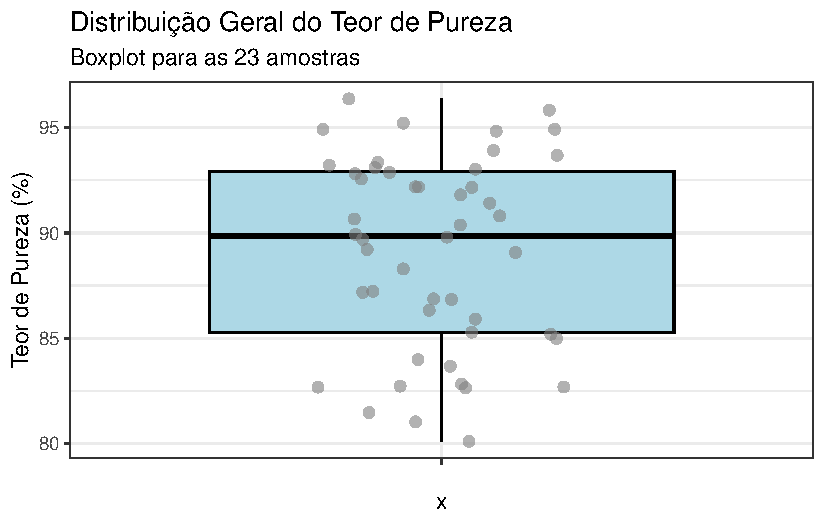
\includegraphics[keepaspectratio]{Controle_de_qualidade--3-_files/figure-pdf/unnamed-chunk-11-1.pdf}}

\begin{Shaded}
\begin{Highlighting}[]
\CommentTok{\# Calcular a diferença absoluta no teor de pureza entre amostras consecutivas}
\NormalTok{tabela\_pureza2 }\OtherTok{\textless{}{-}}\NormalTok{ tabela\_pureza2 }\SpecialCharTok{\%\textgreater{}\%}
  \FunctionTok{mutate}\NormalTok{(}\AttributeTok{Diferenca\_Pureza =} \FunctionTok{abs}\NormalTok{(Teor\_Pureza1 }\SpecialCharTok{{-}} \FunctionTok{mean}\NormalTok{(Teor\_Pureza1)))  }\CommentTok{\# Diferença entre amostras consecutivas}

\CommentTok{\# Selecionar as 5 amostras com a maior diferença no teor de pureza}
\NormalTok{top\_5\_maior\_diferenca }\OtherTok{\textless{}{-}}\NormalTok{ tabela\_pureza2 }\SpecialCharTok{\%\textgreater{}\%}
  \FunctionTok{arrange}\NormalTok{(}\FunctionTok{desc}\NormalTok{(Diferenca\_Pureza)) }\SpecialCharTok{\%\textgreater{}\%}
  \FunctionTok{slice\_head}\NormalTok{(}\AttributeTok{n =} \DecValTok{5}\NormalTok{)}

\CommentTok{\# Calcular a média da diferença}
\NormalTok{media\_diferenca\_maior }\OtherTok{\textless{}{-}} \FunctionTok{mean}\NormalTok{(top\_5\_maior\_diferenca}\SpecialCharTok{$}\NormalTok{Diferenca\_Pureza, }\AttributeTok{na.rm =} \ConstantTok{TRUE}\NormalTok{)}

\CommentTok{\# Criar o gráfico de barras}
\FunctionTok{ggplot}\NormalTok{(top\_5\_maior\_diferenca, }\FunctionTok{aes}\NormalTok{(}\AttributeTok{x =} \FunctionTok{factor}\NormalTok{(Numero\_Amostra1), }\AttributeTok{y =}\NormalTok{ Diferenca\_Pureza)) }\SpecialCharTok{+}
  \FunctionTok{geom\_bar}\NormalTok{(}\AttributeTok{stat =} \StringTok{"identity"}\NormalTok{, }\AttributeTok{fill =} \StringTok{"steelblue"}\NormalTok{, }\AttributeTok{color =} \StringTok{"black"}\NormalTok{) }\SpecialCharTok{+}
  \FunctionTok{geom\_hline}\NormalTok{(}\AttributeTok{yintercept =}\NormalTok{ media\_diferenca\_maior, }\AttributeTok{linetype =} \StringTok{"dashed"}\NormalTok{, }\AttributeTok{color =} \StringTok{"red"}\NormalTok{) }\SpecialCharTok{+}  \CommentTok{\# Linha de média}
  \FunctionTok{labs}\NormalTok{(}\AttributeTok{title =} \StringTok{"As 5 Amostras com Maior Diferença de Pureza"}\NormalTok{,}
       \AttributeTok{subtitle =} \StringTok{"Variação de pureza entre amostras consecutivas"}\NormalTok{,}
       \AttributeTok{x =} \StringTok{"Número da Amostra"}\NormalTok{,}
       \AttributeTok{y =} \StringTok{"Diferença Absoluta no Teor de Pureza"}\NormalTok{) }\SpecialCharTok{+}
  \FunctionTok{theme\_bw}\NormalTok{() }\SpecialCharTok{+}
  \FunctionTok{annotate}\NormalTok{(}\StringTok{"text"}\NormalTok{, }\AttributeTok{x =} \DecValTok{3}\NormalTok{, }\AttributeTok{y =}\NormalTok{ media\_diferenca\_maior }\SpecialCharTok{+} \FloatTok{0.1}\NormalTok{, }\AttributeTok{label =} \FunctionTok{paste}\NormalTok{(}\StringTok{"Média ="}\NormalTok{, }\FunctionTok{round}\NormalTok{(media\_diferenca\_maior, }\DecValTok{2}\NormalTok{)), }\AttributeTok{color =} \StringTok{"red"}\NormalTok{)}
\end{Highlighting}
\end{Shaded}

\pandocbounded{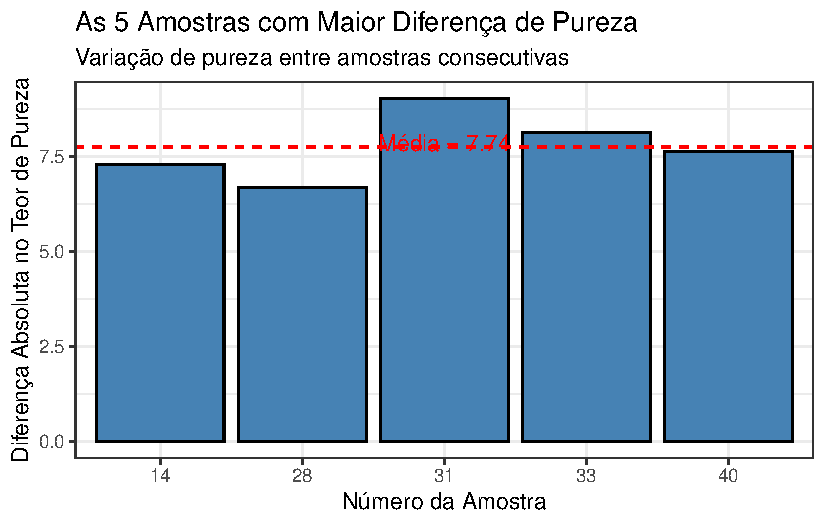
\includegraphics[keepaspectratio]{Controle_de_qualidade--3-_files/figure-pdf/unnamed-chunk-12-1.pdf}}

\begin{Shaded}
\begin{Highlighting}[]
\CommentTok{\# Calcular a diferença absoluta no teor de pureza entre amostras consecutivas}
\NormalTok{tabela\_pureza2 }\OtherTok{\textless{}{-}}\NormalTok{ tabela\_pureza2 }\SpecialCharTok{\%\textgreater{}\%}
  \FunctionTok{mutate}\NormalTok{(}\AttributeTok{Diferenca\_Pureza =} \FunctionTok{abs}\NormalTok{(Teor\_Pureza1 }\SpecialCharTok{{-}} \FunctionTok{mean}\NormalTok{(Teor\_Pureza1)))  }\CommentTok{\# Diferença entre amostras consecutivas}

\CommentTok{\# Selecionar as 5 amostras com a menor diferença no teor de pureza}
\NormalTok{top\_5\_menor\_diferenca }\OtherTok{\textless{}{-}}\NormalTok{ tabela\_pureza2 }\SpecialCharTok{\%\textgreater{}\%}
  \FunctionTok{arrange}\NormalTok{(Diferenca\_Pureza) }\SpecialCharTok{\%\textgreater{}\%}
  \FunctionTok{slice\_head}\NormalTok{(}\AttributeTok{n =} \DecValTok{5}\NormalTok{)}

\CommentTok{\# Calcular a média da diferença}
\NormalTok{media\_diferenca }\OtherTok{\textless{}{-}} \FunctionTok{mean}\NormalTok{(top\_5\_menor\_diferenca}\SpecialCharTok{$}\NormalTok{Diferenca\_Pureza, }\AttributeTok{na.rm =} \ConstantTok{TRUE}\NormalTok{)}

\CommentTok{\# Criar o gráfico de barras}
\FunctionTok{ggplot}\NormalTok{(top\_5\_menor\_diferenca, }\FunctionTok{aes}\NormalTok{(}\AttributeTok{x =} \FunctionTok{factor}\NormalTok{(Numero\_Amostra1), }\AttributeTok{y =}\NormalTok{ Diferenca\_Pureza)) }\SpecialCharTok{+}
  \FunctionTok{geom\_bar}\NormalTok{(}\AttributeTok{stat =} \StringTok{"identity"}\NormalTok{, }\AttributeTok{fill =} \StringTok{"orange"}\NormalTok{, }\AttributeTok{color =} \StringTok{"black"}\NormalTok{) }\SpecialCharTok{+}
  \FunctionTok{geom\_hline}\NormalTok{(}\AttributeTok{yintercept =}\NormalTok{ media\_diferenca, }\AttributeTok{linetype =} \StringTok{"dashed"}\NormalTok{, }\AttributeTok{color =} \StringTok{"red"}\NormalTok{) }\SpecialCharTok{+}  \CommentTok{\# Linha de média}
  \FunctionTok{labs}\NormalTok{(}\AttributeTok{title =} \StringTok{"As 5 Amostras com Menor Diferença de Pureza"}\NormalTok{,}
       \AttributeTok{subtitle =} \StringTok{"Variação de pureza entre amostras consecutivas"}\NormalTok{,}
       \AttributeTok{x =} \StringTok{"Número da Amostra"}\NormalTok{,}
       \AttributeTok{y =} \StringTok{"Diferença Absoluta no Teor de Pureza"}\NormalTok{) }\SpecialCharTok{+}
  \FunctionTok{theme\_bw}\NormalTok{() }\SpecialCharTok{+}
  \FunctionTok{annotate}\NormalTok{(}\StringTok{"text"}\NormalTok{, }\AttributeTok{x =} \DecValTok{3}\NormalTok{, }\AttributeTok{y =}\NormalTok{ media\_diferenca }\SpecialCharTok{+} \FloatTok{0.1}\NormalTok{, }\AttributeTok{label =} \FunctionTok{paste}\NormalTok{(}\StringTok{"Média ="}\NormalTok{, }\FunctionTok{round}\NormalTok{(media\_diferenca, }\DecValTok{2}\NormalTok{)), }\AttributeTok{color =} \StringTok{"red"}\NormalTok{)}
\end{Highlighting}
\end{Shaded}

\pandocbounded{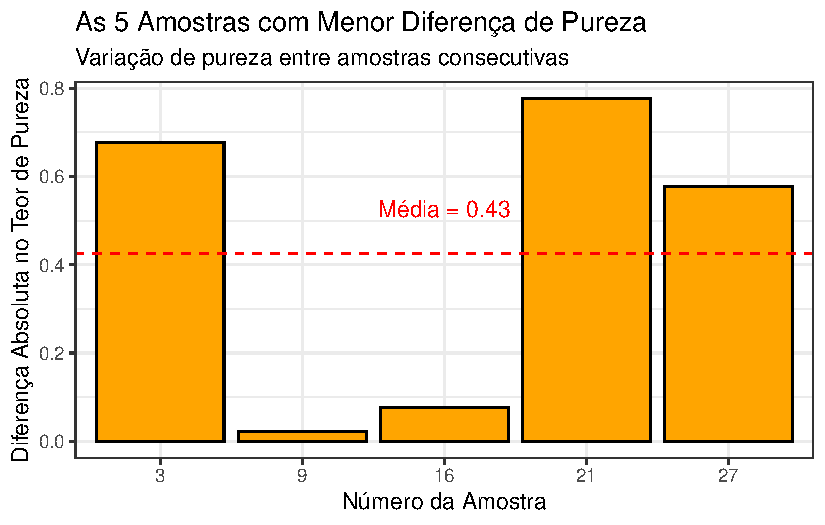
\includegraphics[keepaspectratio]{Controle_de_qualidade--3-_files/figure-pdf/unnamed-chunk-13-1.pdf}}

\subsubsection{Resumo dos Dados}\label{resumo-dos-dados}

\begin{Shaded}
\begin{Highlighting}[]
\FunctionTok{suppressMessages}\NormalTok{(}\FunctionTok{library}\NormalTok{(kableExtra))}

\CommentTok{\# Calcular o resumo estatístico para a coluna "Teor\_Pureza" e "Amplitude\_Movel"}
\NormalTok{resumo2 }\OtherTok{\textless{}{-}} \FunctionTok{summary}\NormalTok{(}\FunctionTok{na.omit}\NormalTok{(tabela\_pureza2[, }\FunctionTok{c}\NormalTok{(}\DecValTok{2}\NormalTok{, }\DecValTok{3}\NormalTok{)])); resumo2}
\end{Highlighting}
\end{Shaded}

\begin{verbatim}
  Teor_Pureza1   Amplitude_Movel1
 Min.   :80.10   Min.   : 0.400  
 1st Qu.:85.25   1st Qu.: 1.300  
 Median :89.80   Median : 2.200  
 Mean   :89.04   Mean   : 2.843  
 3rd Qu.:92.90   3rd Qu.: 4.050  
 Max.   :96.40   Max.   :12.200  
\end{verbatim}

\subsubsection{Gráfico AM: calcular o limite inferior e o
superior}\label{gruxe1fico-am-calcular-o-limite-inferior-e-o-superior}

\begin{Shaded}
\begin{Highlighting}[]
\CommentTok{\# Calcular os limites de controle para os gráficos AM}
\NormalTok{D3 }\OtherTok{=} \DecValTok{0}\NormalTok{ ; D4 }\OtherTok{=} \FloatTok{3.267} 

\CommentTok{\# Cálculo dos limites de controle para o gráfico AM}
\NormalTok{AM\_bar }\OtherTok{\textless{}{-}} \FunctionTok{mean}\NormalTok{(tabela\_pureza2}\SpecialCharTok{$}\NormalTok{Amplitude\_Movel1, }\AttributeTok{na.rm =} \ConstantTok{TRUE}\NormalTok{)  }\CommentTok{\# Média da Amplitude Móvel}
\NormalTok{LSC\_AM }\OtherTok{\textless{}{-}}\NormalTok{ D4 }\SpecialCharTok{*}\NormalTok{ AM\_bar}
\NormalTok{LIC\_AM }\OtherTok{\textless{}{-}}\NormalTok{ D3 }\SpecialCharTok{*}\NormalTok{ AM\_bar}
\FunctionTok{cat}\NormalTok{(}\StringTok{"LSC AM:"}\NormalTok{, LSC\_AM, }\StringTok{"}\SpecialCharTok{\textbackslash{}n}\StringTok{"}\NormalTok{)}
\end{Highlighting}
\end{Shaded}

\begin{verbatim}
LSC AM: 9.286621 
\end{verbatim}

\begin{Shaded}
\begin{Highlighting}[]
\FunctionTok{cat}\NormalTok{(}\StringTok{"LIC AM:"}\NormalTok{, LIC\_AM, }\StringTok{"}\SpecialCharTok{\textbackslash{}n\textbackslash{}n}\StringTok{"}\NormalTok{)}
\end{Highlighting}
\end{Shaded}

\begin{verbatim}
LIC AM: 0 
\end{verbatim}

\subsubsection{Gráfico X: calcular o limite inferior e o
superior}\label{gruxe1fico-x-calcular-o-limite-inferior-e-o-superior}

\begin{Shaded}
\begin{Highlighting}[]
\CommentTok{\# Cálculo dos limites de controle para o gráfico X}
\NormalTok{d2 }\OtherTok{=} \FloatTok{1.128}

\NormalTok{X\_bar }\OtherTok{\textless{}{-}} \FunctionTok{mean}\NormalTok{(tabela\_pureza2}\SpecialCharTok{$}\NormalTok{Teor\_Pureza1, }\AttributeTok{na.rm =} \ConstantTok{TRUE}\NormalTok{)  }\CommentTok{\# Média do Teor de Pureza}
\NormalTok{LSC\_X }\OtherTok{\textless{}{-}}\NormalTok{ X\_bar }\SpecialCharTok{+} \DecValTok{3} \SpecialCharTok{*}\NormalTok{ (AM\_bar }\SpecialCharTok{/}\NormalTok{ d2)}
\NormalTok{LIC\_X }\OtherTok{\textless{}{-}}\NormalTok{ X\_bar }\SpecialCharTok{{-}} \DecValTok{3} \SpecialCharTok{*}\NormalTok{ (AM\_bar }\SpecialCharTok{/}\NormalTok{ d2)}
\FunctionTok{cat}\NormalTok{(}\StringTok{"LSC X:"}\NormalTok{, LSC\_X, }\StringTok{"}\SpecialCharTok{\textbackslash{}n}\StringTok{"}\NormalTok{)}
\end{Highlighting}
\end{Shaded}

\begin{verbatim}
LSC X: 96.6829 
\end{verbatim}

\begin{Shaded}
\begin{Highlighting}[]
\FunctionTok{cat}\NormalTok{(}\StringTok{"LIC X:"}\NormalTok{, LIC\_X, }\StringTok{"}\SpecialCharTok{\textbackslash{}n}\StringTok{"}\NormalTok{)}
\end{Highlighting}
\end{Shaded}

\begin{verbatim}
LIC X: 81.56293 
\end{verbatim}

\subsubsection{Análise no Gráfico da Amplitude
Móvel}\label{anuxe1lise-no-gruxe1fico-da-amplitude-muxf3vel}

\subsubsection{O Limite Médio (LM) é obtido a partir da média geral das
amostras. Para calcular os Limites de Controle da média, utiliza-se a
constante
d2.}\label{o-limite-muxe9dio-lm-uxe9-obtido-a-partir-da-muxe9dia-geral-das-amostras.-para-calcular-os-limites-de-controle-da-muxe9dia-utiliza-se-a-constante-d2.-1}

\begin{Shaded}
\begin{Highlighting}[]
\CommentTok{\# Gráfico de Controle AM interativo}
\NormalTok{grafico\_AM }\OtherTok{\textless{}{-}} \FunctionTok{plot\_ly}\NormalTok{(}\AttributeTok{x =} \FunctionTok{seq\_along}\NormalTok{(tabela\_pureza2}\SpecialCharTok{$}\NormalTok{Amplitude\_Movel1), }
                      \AttributeTok{y =}\NormalTok{ tabela\_pureza2}\SpecialCharTok{$}\NormalTok{Amplitude\_Movel1, }
                      \AttributeTok{type =} \StringTok{\textquotesingle{}scatter\textquotesingle{}}\NormalTok{, }
                      \AttributeTok{mode =} \StringTok{\textquotesingle{}lines+markers\textquotesingle{}}\NormalTok{, }
                      \AttributeTok{name =} \StringTok{\textquotesingle{}AM\textquotesingle{}}\NormalTok{) }\SpecialCharTok{\%\textgreater{}\%}
  \FunctionTok{add\_trace}\NormalTok{(}\AttributeTok{y =} \FunctionTok{rep}\NormalTok{(AM\_bar, }\FunctionTok{length}\NormalTok{(tabela\_pureza2}\SpecialCharTok{$}\NormalTok{Amplitude\_Movel1)), }
            \AttributeTok{mode =} \StringTok{"lines"}\NormalTok{, }
            \AttributeTok{name =} \StringTok{"Média AM"}\NormalTok{, }
            \AttributeTok{line =} \FunctionTok{list}\NormalTok{(}\AttributeTok{color =} \StringTok{"blue"}\NormalTok{)) }\SpecialCharTok{\%\textgreater{}\%}
  \FunctionTok{add\_trace}\NormalTok{(}\AttributeTok{y =} \FunctionTok{rep}\NormalTok{(LSC\_AM, }\FunctionTok{length}\NormalTok{(tabela\_pureza2}\SpecialCharTok{$}\NormalTok{Amplitude\_Movel1)), }
            \AttributeTok{mode =} \StringTok{"lines"}\NormalTok{, }
            \AttributeTok{name =} \StringTok{"LSC"}\NormalTok{, }
            \AttributeTok{line =} \FunctionTok{list}\NormalTok{(}\AttributeTok{color =} \StringTok{"red"}\NormalTok{, }\AttributeTok{dash =} \StringTok{\textquotesingle{}dash\textquotesingle{}}\NormalTok{)) }\SpecialCharTok{\%\textgreater{}\%}
  \FunctionTok{add\_trace}\NormalTok{(}\AttributeTok{y =} \FunctionTok{rep}\NormalTok{(LIC\_AM, }\FunctionTok{length}\NormalTok{(tabela\_pureza2}\SpecialCharTok{$}\NormalTok{Amplitude\_Movel1)), }
            \AttributeTok{mode =} \StringTok{"lines"}\NormalTok{, }
            \AttributeTok{name =} \StringTok{"LIC"}\NormalTok{, }
            \AttributeTok{line =} \FunctionTok{list}\NormalTok{(}\AttributeTok{color =} \StringTok{"red"}\NormalTok{, }\AttributeTok{dash =} \StringTok{\textquotesingle{}dash\textquotesingle{}}\NormalTok{)) }\SpecialCharTok{\%\textgreater{}\%}
  \FunctionTok{layout}\NormalTok{(}\AttributeTok{title =} \StringTok{"Gráfico da Amplitude Móvel (AM)"}\NormalTok{,}
         \AttributeTok{xaxis =} \FunctionTok{list}\NormalTok{(}\AttributeTok{title =} \StringTok{"Número da Amostra"}\NormalTok{),}
         \AttributeTok{yaxis =} \FunctionTok{list}\NormalTok{(}\AttributeTok{title =} \StringTok{"AM"}\NormalTok{))}

\CommentTok{\# Exibir o gráfico AM}
\NormalTok{grafico\_AM}
\end{Highlighting}
\end{Shaded}

\begin{verbatim}
file:///C:/Users/fabia/AppData/Local/Temp/Rtmp4KpvhV/file2b1458691a2b/widget2b1487bfe.html screenshot completed
\end{verbatim}

\pandocbounded{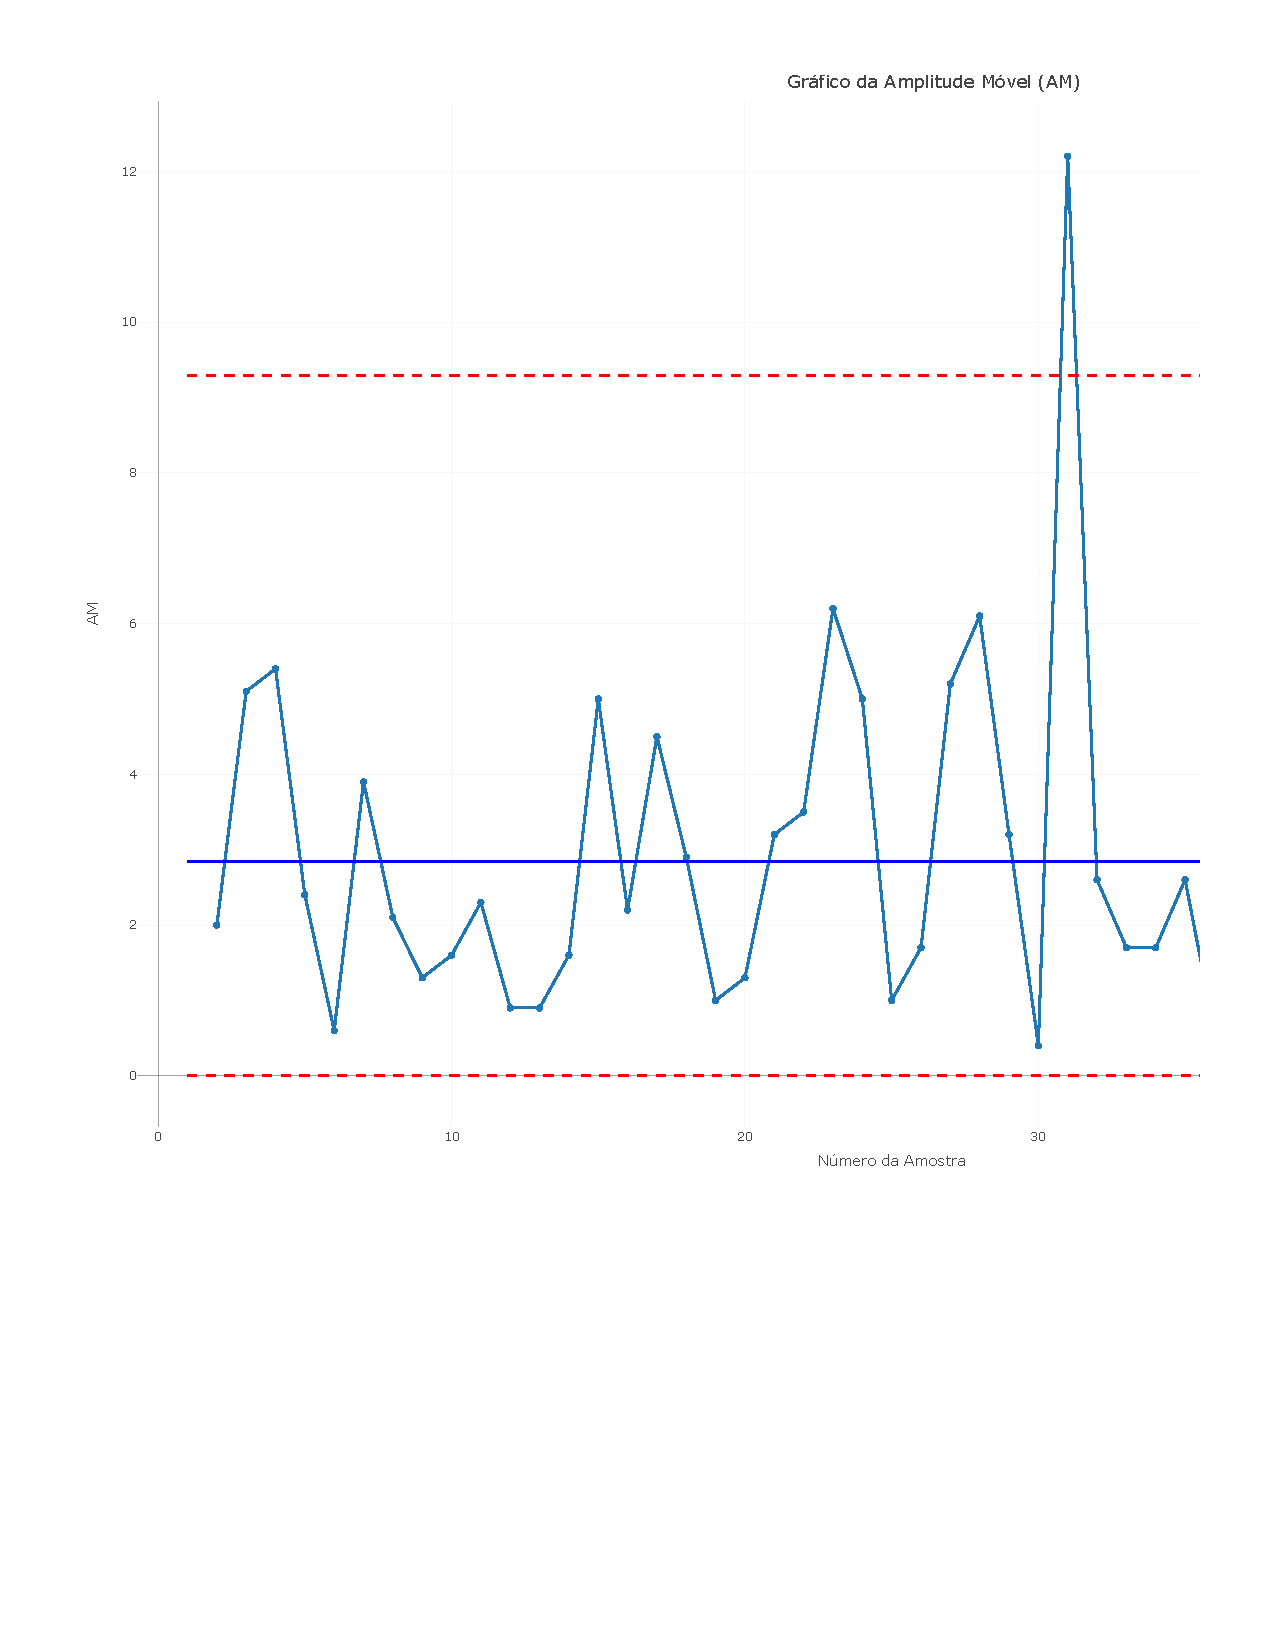
\includegraphics[keepaspectratio]{Controle_de_qualidade--3-_files/figure-pdf/unnamed-chunk-17-1.pdf}}

\subsubsection{O gráfico da amplitude móvel indicou a presença de uma
amostra fora de controle, isso indica a presença de amostras fora de
controle no gráfico de medidas individuais indica que o processo não
está estável e dentro dos limites esperados, com variações
presentes.}\label{o-gruxe1fico-da-amplitude-muxf3vel-indicou-a-presenuxe7a-de-uma-amostra-fora-de-controle-isso-indica-a-presenuxe7a-de-amostras-fora-de-controle-no-gruxe1fico-de-medidas-individuais-indica-que-o-processo-nuxe3o-estuxe1-estuxe1vel-e-dentro-dos-limites-esperados-com-variauxe7uxf5es-presentes.}

\subsubsection{Análise no Gráfico para medidas
individuais}\label{anuxe1lise-no-gruxe1fico-para-medidas-individuais}

\begin{Shaded}
\begin{Highlighting}[]
\CommentTok{\# Gráfico de Controle X̄ interativo}
\NormalTok{grafico\_X }\OtherTok{\textless{}{-}} \FunctionTok{plot\_ly}\NormalTok{(}\AttributeTok{x =} \FunctionTok{seq\_along}\NormalTok{(tabela\_pureza2}\SpecialCharTok{$}\NormalTok{Teor\_Pureza1), }
                     \AttributeTok{y =}\NormalTok{ tabela\_pureza2}\SpecialCharTok{$}\NormalTok{Teor\_Pureza1, }
                     \AttributeTok{type =} \StringTok{\textquotesingle{}scatter\textquotesingle{}}\NormalTok{, }
                     \AttributeTok{mode =} \StringTok{\textquotesingle{}lines+markers\textquotesingle{}}\NormalTok{, }
                     \AttributeTok{name =} \StringTok{\textquotesingle{}Média das Amostras\textquotesingle{}}\NormalTok{) }\SpecialCharTok{\%\textgreater{}\%}
  \FunctionTok{add\_trace}\NormalTok{(}\AttributeTok{y =} \FunctionTok{rep}\NormalTok{(X\_bar, }\FunctionTok{length}\NormalTok{(tabela\_pureza2}\SpecialCharTok{$}\NormalTok{Teor\_Pureza1)), }
            \AttributeTok{mode =} \StringTok{"lines"}\NormalTok{, }
            \AttributeTok{name =} \StringTok{"Média X̄"}\NormalTok{, }
            \AttributeTok{line =} \FunctionTok{list}\NormalTok{(}\AttributeTok{color =} \StringTok{"blue"}\NormalTok{)) }\SpecialCharTok{\%\textgreater{}\%}
  \FunctionTok{add\_trace}\NormalTok{(}\AttributeTok{y =} \FunctionTok{rep}\NormalTok{(LSC\_X, }\FunctionTok{length}\NormalTok{(tabela\_pureza2}\SpecialCharTok{$}\NormalTok{Teor\_Pureza1)), }
            \AttributeTok{mode =} \StringTok{"lines"}\NormalTok{, }
            \AttributeTok{name =} \StringTok{"LSC"}\NormalTok{, }
            \AttributeTok{line =} \FunctionTok{list}\NormalTok{(}\AttributeTok{color =} \StringTok{"red"}\NormalTok{, }\AttributeTok{dash =} \StringTok{\textquotesingle{}dash\textquotesingle{}}\NormalTok{)) }\SpecialCharTok{\%\textgreater{}\%}
  \FunctionTok{add\_trace}\NormalTok{(}\AttributeTok{y =} \FunctionTok{rep}\NormalTok{(LIC\_X, }\FunctionTok{length}\NormalTok{(tabela\_pureza2}\SpecialCharTok{$}\NormalTok{Teor\_Pureza1)), }
            \AttributeTok{mode =} \StringTok{"lines"}\NormalTok{, }
            \AttributeTok{name =} \StringTok{"LIC"}\NormalTok{, }
            \AttributeTok{line =} \FunctionTok{list}\NormalTok{(}\AttributeTok{color =} \StringTok{"red"}\NormalTok{, }\AttributeTok{dash =} \StringTok{\textquotesingle{}dash\textquotesingle{}}\NormalTok{)) }\SpecialCharTok{\%\textgreater{}\%}
  \FunctionTok{layout}\NormalTok{(}\AttributeTok{title =} \StringTok{"Gráfico para Medidas Individuais"}\NormalTok{,}
         \AttributeTok{xaxis =} \FunctionTok{list}\NormalTok{(}\AttributeTok{title =} \StringTok{"Número da Amostra"}\NormalTok{),}
         \AttributeTok{yaxis =} \FunctionTok{list}\NormalTok{(}\AttributeTok{title =} \StringTok{"X"}\NormalTok{))}

\CommentTok{\# Exibir o gráfico X}
\NormalTok{grafico\_X}
\end{Highlighting}
\end{Shaded}

\begin{verbatim}
file:///C:/Users/fabia/AppData/Local/Temp/Rtmp4KpvhV/file2b147db15d75/widget2b1413005e47.html screenshot completed
\end{verbatim}

\pandocbounded{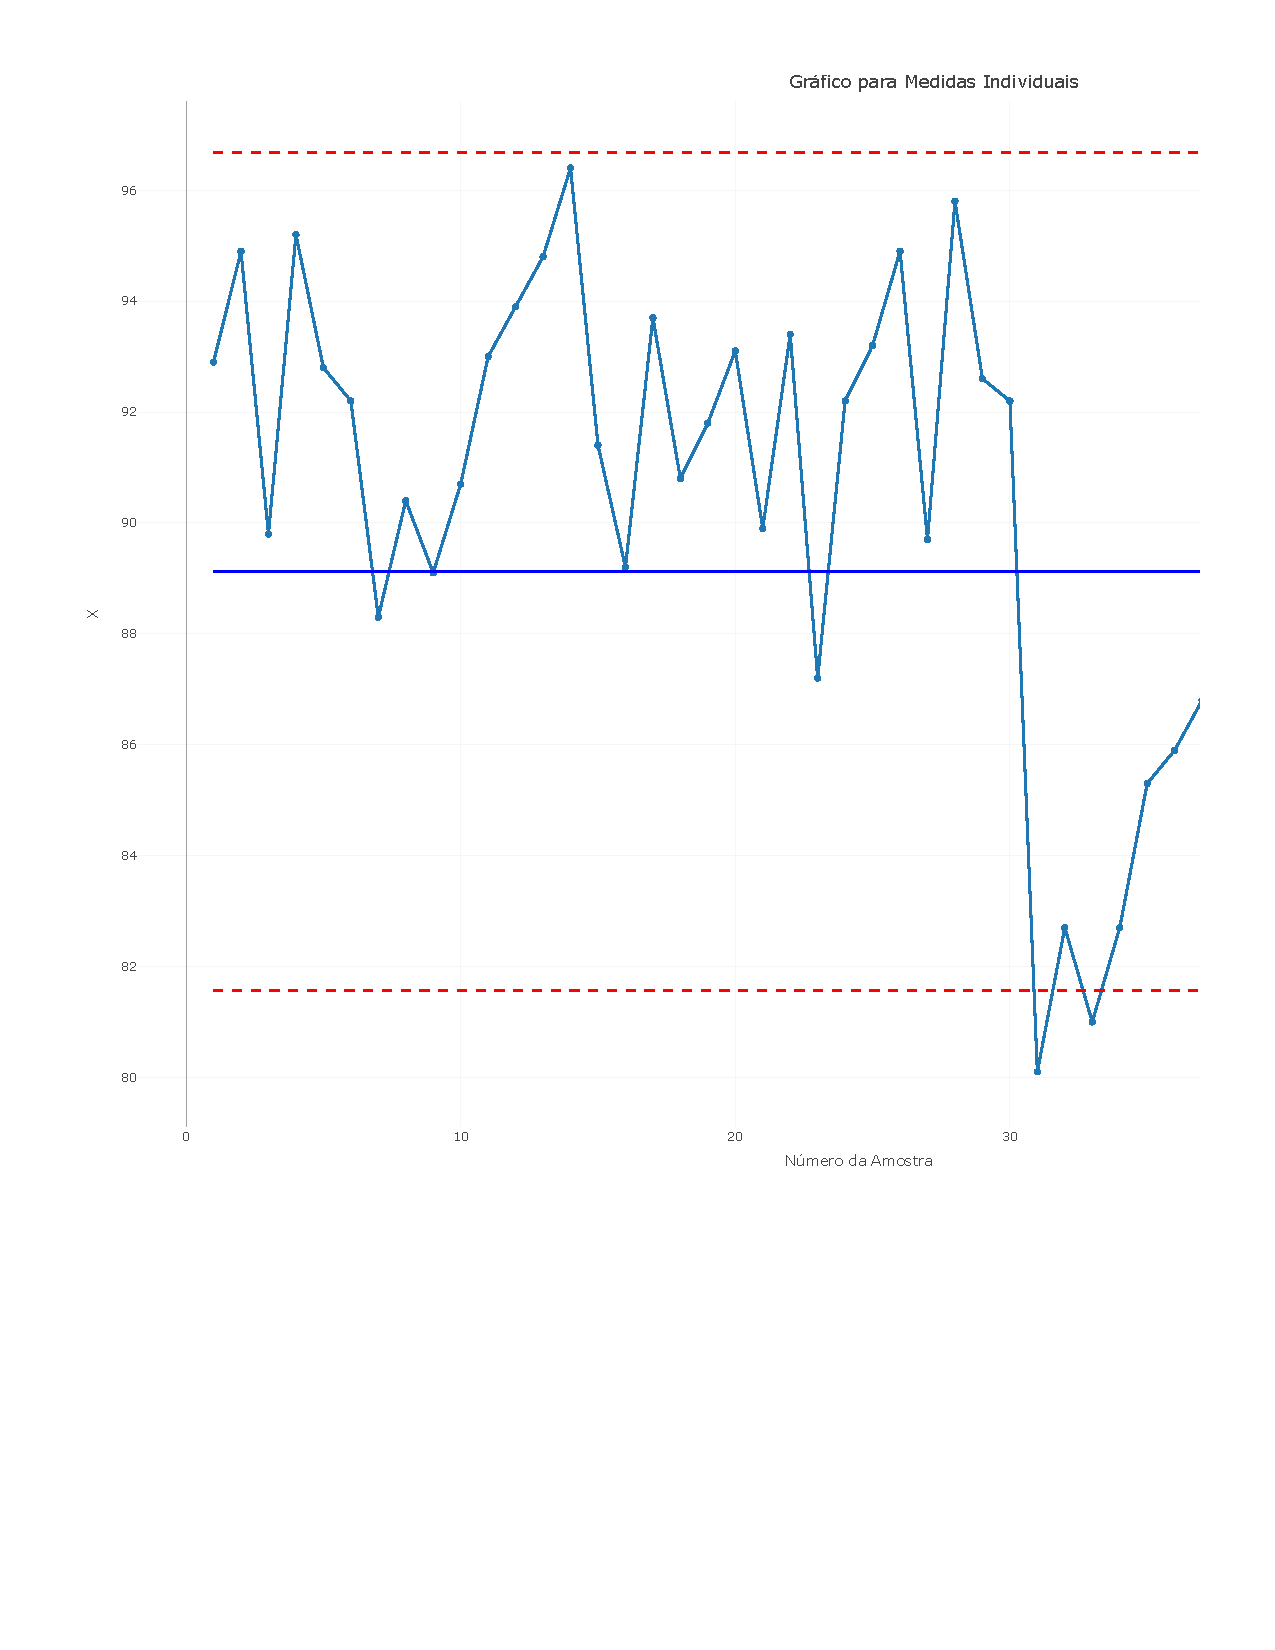
\includegraphics[keepaspectratio]{Controle_de_qualidade--3-_files/figure-pdf/unnamed-chunk-18-1.pdf}}

\subsubsection{O gráfico das medidas individuais mostrou a presença de
algumas amostras que estão fora de
controle.}\label{o-gruxe1fico-das-medidas-individuais-mostrou-a-presenuxe7a-de-algumas-amostras-que-estuxe3o-fora-de-controle.}

\subsubsection{Identificar amostras que fora de controle no gráfico
Amplitude
móvel}\label{identificar-amostras-que-fora-de-controle-no-gruxe1fico-amplitude-muxf3vel}

\begin{Shaded}
\begin{Highlighting}[]
\NormalTok{fora\_controle\_AM }\OtherTok{\textless{}{-}} \FunctionTok{which}\NormalTok{(tabela\_pureza2}\SpecialCharTok{$}\NormalTok{Amplitude\_Movel1 }\SpecialCharTok{\textgreater{}}\NormalTok{ LSC\_AM }\SpecialCharTok{|}\NormalTok{ tabela\_pureza2}\SpecialCharTok{$}\NormalTok{Amplitude\_Movel1 }\SpecialCharTok{\textless{}}\NormalTok{ LIC\_AM); }\FunctionTok{print}\NormalTok{(fora\_controle\_AM)}
\end{Highlighting}
\end{Shaded}

\begin{verbatim}
[1] 31
\end{verbatim}

\begin{Shaded}
\begin{Highlighting}[]
\NormalTok{fora\_controle\_X }\OtherTok{\textless{}{-}} \FunctionTok{which}\NormalTok{(tabela\_pureza2}\SpecialCharTok{$}\NormalTok{Teor\_Pureza1 }\SpecialCharTok{\textgreater{}}\NormalTok{ LSC\_X }\SpecialCharTok{|}\NormalTok{ tabela\_pureza2}\SpecialCharTok{$}\NormalTok{Teor\_Pureza1 }\SpecialCharTok{\textless{}}\NormalTok{ LIC\_X); }\FunctionTok{print}\NormalTok{(fora\_controle\_AM)}
\end{Highlighting}
\end{Shaded}

\begin{verbatim}
[1] 31
\end{verbatim}

\subsubsection{Tabela corrigida sem valores os mais
diferentes/discrepantes}\label{tabela-corrigida-sem-valores-os-mais-diferentesdiscrepantes}

\begin{Shaded}
\begin{Highlighting}[]
\CommentTok{\# Remover amostras fora de controle}
\NormalTok{tabela\_pureza\_corrigida }\OtherTok{\textless{}{-}}\NormalTok{ tabela\_pureza2[}\SpecialCharTok{{-}}\FunctionTok{c}\NormalTok{(fora\_controle\_AM, fora\_controle\_X), ];}
\end{Highlighting}
\end{Shaded}

\begin{Shaded}
\begin{Highlighting}[]
\CommentTok{\# Refazer os cálculos com os dados corrigidos}
\NormalTok{AM\_bar\_corrigido }\OtherTok{\textless{}{-}} \FunctionTok{mean}\NormalTok{(tabela\_pureza\_corrigida}\SpecialCharTok{$}\NormalTok{Amplitude\_Movel, }\AttributeTok{na.rm =} \ConstantTok{TRUE}\NormalTok{)  }
\NormalTok{LSC\_AM\_corrigido }\OtherTok{\textless{}{-}}\NormalTok{ D4 }\SpecialCharTok{*}\NormalTok{ AM\_bar\_corrigido}
\NormalTok{LIC\_AM\_corrigido }\OtherTok{\textless{}{-}}\NormalTok{ D3 }\SpecialCharTok{*}\NormalTok{ AM\_bar\_corrigido}
\end{Highlighting}
\end{Shaded}

\begin{Shaded}
\begin{Highlighting}[]
\CommentTok{\# Gráfico AM corrigido}
\NormalTok{grafico\_AM\_corrigido }\OtherTok{\textless{}{-}} \FunctionTok{plot\_ly}\NormalTok{(}\AttributeTok{x =} \FunctionTok{seq\_along}\NormalTok{(tabela\_pureza\_corrigida}\SpecialCharTok{$}\NormalTok{Amplitude\_Movel), }
                                \AttributeTok{y =}\NormalTok{ tabela\_pureza\_corrigida}\SpecialCharTok{$}\NormalTok{Amplitude\_Movel, }
                                \AttributeTok{type =} \StringTok{\textquotesingle{}scatter\textquotesingle{}}\NormalTok{, }
                                \AttributeTok{mode =} \StringTok{\textquotesingle{}lines+markers\textquotesingle{}}\NormalTok{, }
                                \AttributeTok{name =} \StringTok{\textquotesingle{}AM\textquotesingle{}}\NormalTok{) }\SpecialCharTok{\%\textgreater{}\%}
  \FunctionTok{add\_trace}\NormalTok{(}\AttributeTok{y =} \FunctionTok{rep}\NormalTok{(AM\_bar\_corrigido, }\FunctionTok{length}\NormalTok{(tabela\_pureza\_corrigida}\SpecialCharTok{$}\NormalTok{Amplitude\_Movel)), }
            \AttributeTok{mode =} \StringTok{"lines"}\NormalTok{, }
            \AttributeTok{name =} \StringTok{"Média AM"}\NormalTok{, }
            \AttributeTok{line =} \FunctionTok{list}\NormalTok{(}\AttributeTok{color =} \StringTok{"blue"}\NormalTok{)) }\SpecialCharTok{\%\textgreater{}\%}
  \FunctionTok{add\_trace}\NormalTok{(}\AttributeTok{y =} \FunctionTok{rep}\NormalTok{(LSC\_AM\_corrigido, }\FunctionTok{length}\NormalTok{(tabela\_pureza\_corrigida}\SpecialCharTok{$}\NormalTok{Amplitude\_Movel)), }
            \AttributeTok{mode =} \StringTok{"lines"}\NormalTok{, }
            \AttributeTok{name =} \StringTok{"LSC"}\NormalTok{, }
            \AttributeTok{line =} \FunctionTok{list}\NormalTok{(}\AttributeTok{color =} \StringTok{"red"}\NormalTok{, }\AttributeTok{dash =} \StringTok{\textquotesingle{}dash\textquotesingle{}}\NormalTok{)) }\SpecialCharTok{\%\textgreater{}\%}
  \FunctionTok{add\_trace}\NormalTok{(}\AttributeTok{y =} \FunctionTok{rep}\NormalTok{(LIC\_AM\_corrigido, }\FunctionTok{length}\NormalTok{(tabela\_pureza\_corrigida}\SpecialCharTok{$}\NormalTok{Amplitude\_Movel)), }
            \AttributeTok{mode =} \StringTok{"lines"}\NormalTok{, }
            \AttributeTok{name =} \StringTok{"LIC"}\NormalTok{, }
            \AttributeTok{line =} \FunctionTok{list}\NormalTok{(}\AttributeTok{color =} \StringTok{"red"}\NormalTok{, }\AttributeTok{dash =} \StringTok{\textquotesingle{}dash\textquotesingle{}}\NormalTok{)) }\SpecialCharTok{\%\textgreater{}\%}
  \FunctionTok{layout}\NormalTok{(}\AttributeTok{title =} \StringTok{"Gráfico da Amplitude Móvel (AM) {-} Corrigido"}\NormalTok{,}
         \AttributeTok{xaxis =} \FunctionTok{list}\NormalTok{(}\AttributeTok{title =} \StringTok{"Número da Amostra"}\NormalTok{),}
         \AttributeTok{yaxis =} \FunctionTok{list}\NormalTok{(}\AttributeTok{title =} \StringTok{"AM"}\NormalTok{))}

\NormalTok{grafico\_AM\_corrigido}
\end{Highlighting}
\end{Shaded}

\begin{verbatim}
file:///C:/Users/fabia/AppData/Local/Temp/Rtmp4KpvhV/file2b1473101a11/widget2b1425c36ffe.html screenshot completed
\end{verbatim}

\pandocbounded{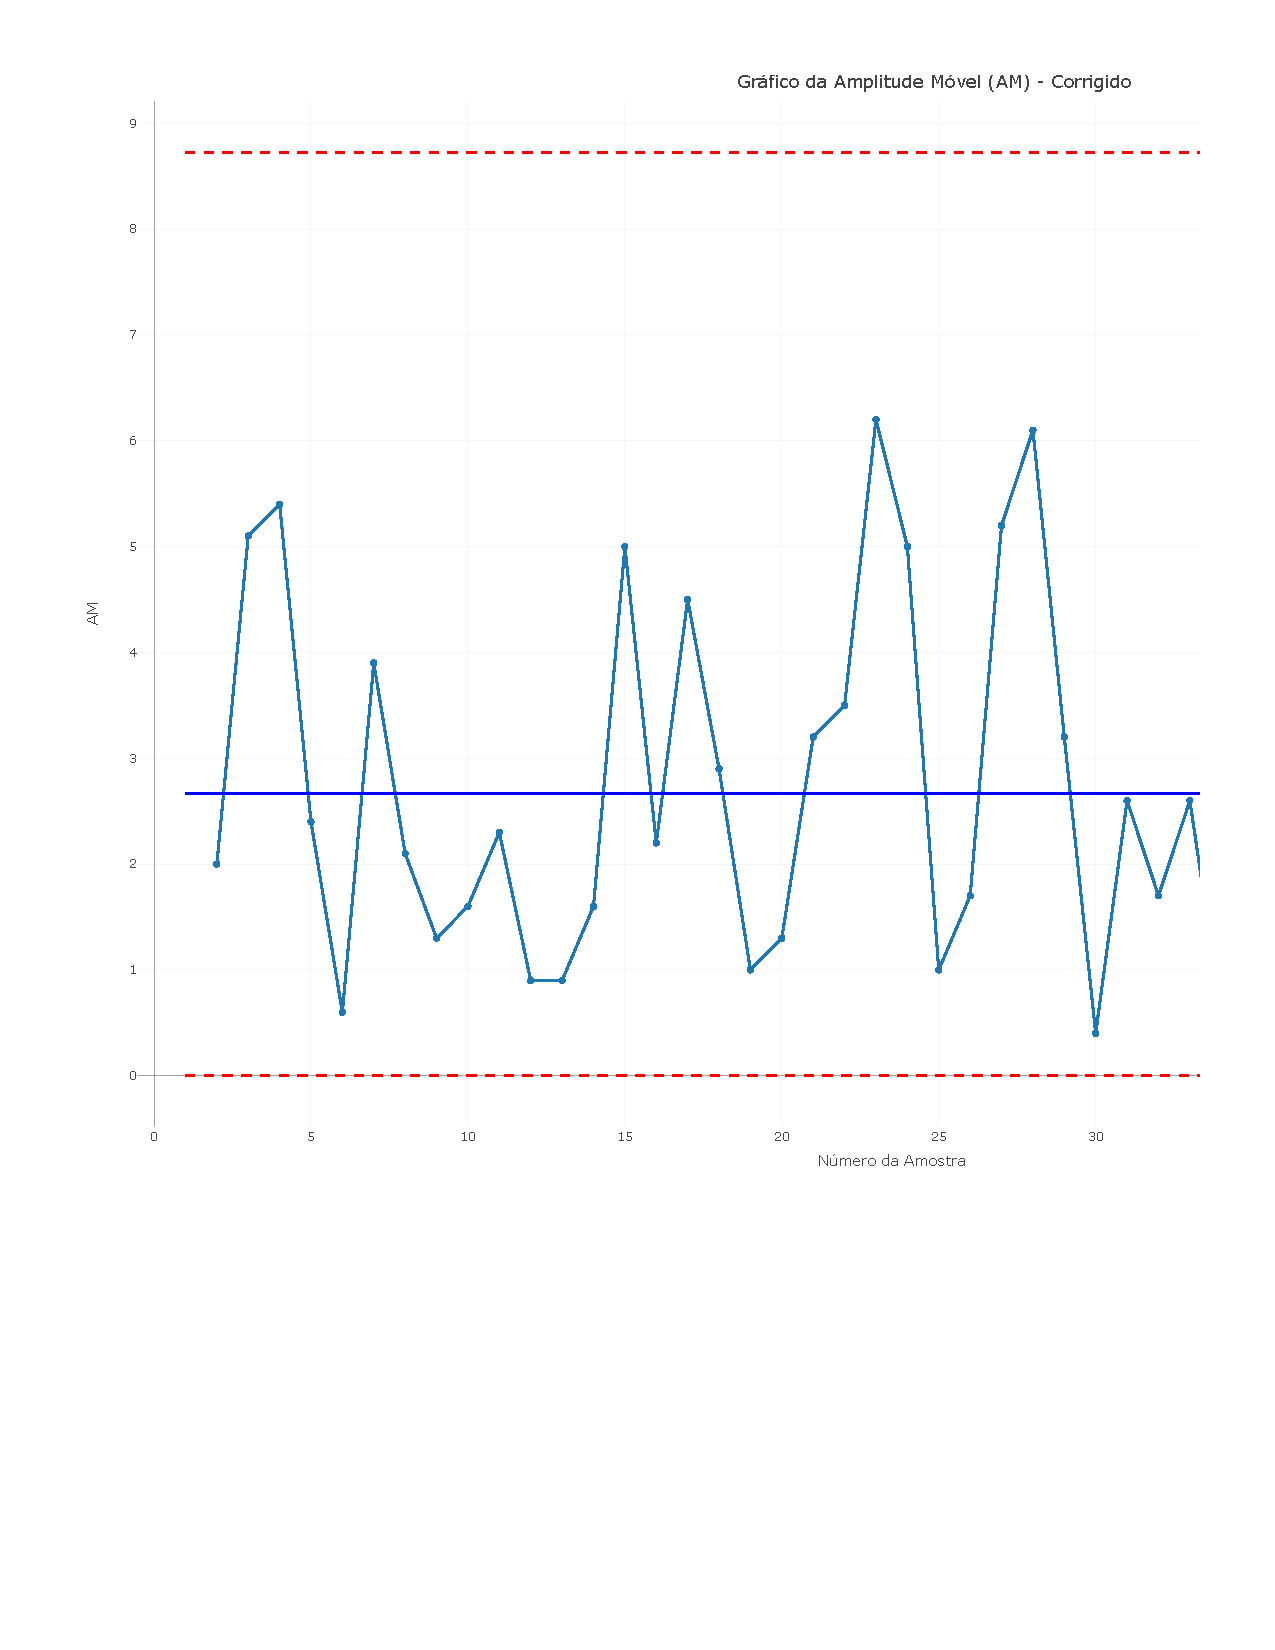
\includegraphics[keepaspectratio]{Controle_de_qualidade--3-_files/figure-pdf/unnamed-chunk-23-1.pdf}}

\begin{Shaded}
\begin{Highlighting}[]
\CommentTok{\# Refazer os cálculos com os dados corrigidos}
\NormalTok{X\_bar\_corrigido }\OtherTok{\textless{}{-}} \FunctionTok{mean}\NormalTok{(tabela\_pureza\_corrigida}\SpecialCharTok{$}\NormalTok{Teor\_Pureza, }\AttributeTok{na.rm =} \ConstantTok{TRUE}\NormalTok{)  }
\NormalTok{LSC\_X\_corrigido }\OtherTok{\textless{}{-}}\NormalTok{ X\_bar\_corrigido }\SpecialCharTok{+} \DecValTok{3} \SpecialCharTok{*}\NormalTok{ (AM\_bar\_corrigido }\SpecialCharTok{/}\NormalTok{ d2)}
\NormalTok{LIC\_X\_corrigido }\OtherTok{\textless{}{-}}\NormalTok{ X\_bar\_corrigido }\SpecialCharTok{{-}} \DecValTok{3} \SpecialCharTok{*}\NormalTok{ (AM\_bar\_corrigido }\SpecialCharTok{/}\NormalTok{ d2)}
\FunctionTok{print}\NormalTok{(LSC\_X\_corrigido)}
\end{Highlighting}
\end{Shaded}

\begin{verbatim}
[1] 96.77561
\end{verbatim}

\begin{Shaded}
\begin{Highlighting}[]
\FunctionTok{print}\NormalTok{(LIC\_X\_corrigido)}
\end{Highlighting}
\end{Shaded}

\begin{verbatim}
[1] 82.57106
\end{verbatim}

\begin{Shaded}
\begin{Highlighting}[]
\NormalTok{grafico\_X\_corrigido }\OtherTok{\textless{}{-}} \FunctionTok{plot\_ly}\NormalTok{(}\AttributeTok{x =} \FunctionTok{seq\_along}\NormalTok{(tabela\_pureza\_corrigida}\SpecialCharTok{$}\NormalTok{Teor\_Pureza), }
                               \AttributeTok{y =}\NormalTok{ tabela\_pureza\_corrigida}\SpecialCharTok{$}\NormalTok{Teor\_Pureza, }
                               \AttributeTok{type =} \StringTok{\textquotesingle{}scatter\textquotesingle{}}\NormalTok{, }
                               \AttributeTok{mode =} \StringTok{\textquotesingle{}lines+markers\textquotesingle{}}\NormalTok{, }
                               \AttributeTok{name =} \StringTok{\textquotesingle{}Média das Amostras\textquotesingle{}}\NormalTok{) }\SpecialCharTok{\%\textgreater{}\%}
  \FunctionTok{add\_trace}\NormalTok{(}\AttributeTok{y =} \FunctionTok{rep}\NormalTok{(X\_bar\_corrigido, }\FunctionTok{length}\NormalTok{(tabela\_pureza\_corrigida}\SpecialCharTok{$}\NormalTok{Teor\_Pureza)), }
            \AttributeTok{mode =} \StringTok{"lines"}\NormalTok{, }
            \AttributeTok{name =} \StringTok{"Média X̄"}\NormalTok{, }
            \AttributeTok{line =} \FunctionTok{list}\NormalTok{(}\AttributeTok{color =} \StringTok{"blue"}\NormalTok{)) }\SpecialCharTok{\%\textgreater{}\%}
  \FunctionTok{add\_trace}\NormalTok{(}\AttributeTok{y =} \FunctionTok{rep}\NormalTok{(LSC\_X\_corrigido, }\FunctionTok{length}\NormalTok{(tabela\_pureza\_corrigida}\SpecialCharTok{$}\NormalTok{Teor\_Pureza)), }
            \AttributeTok{mode =} \StringTok{"lines"}\NormalTok{, }
            \AttributeTok{name =} \StringTok{"LSC"}\NormalTok{, }
            \AttributeTok{line =} \FunctionTok{list}\NormalTok{(}\AttributeTok{color =} \StringTok{"red"}\NormalTok{, }\AttributeTok{dash =} \StringTok{\textquotesingle{}dash\textquotesingle{}}\NormalTok{)) }\SpecialCharTok{\%\textgreater{}\%}
  \FunctionTok{add\_trace}\NormalTok{(}\AttributeTok{y =} \FunctionTok{rep}\NormalTok{(LIC\_X\_corrigido, }\FunctionTok{length}\NormalTok{(tabela\_pureza\_corrigida}\SpecialCharTok{$}\NormalTok{Teor\_Pureza)), }
            \AttributeTok{mode =} \StringTok{"lines"}\NormalTok{, }
            \AttributeTok{name =} \StringTok{"LIC"}\NormalTok{, }
            \AttributeTok{line =} \FunctionTok{list}\NormalTok{(}\AttributeTok{color =} \StringTok{"red"}\NormalTok{, }\AttributeTok{dash =} \StringTok{\textquotesingle{}dash\textquotesingle{}}\NormalTok{)) }\SpecialCharTok{\%\textgreater{}\%}
  \FunctionTok{layout}\NormalTok{(}\AttributeTok{title =} \StringTok{"Gráfico para Medidas Individuais {-} Corrigido"}\NormalTok{,}
         \AttributeTok{xaxis =} \FunctionTok{list}\NormalTok{(}\AttributeTok{title =} \StringTok{"Número da Amostra"}\NormalTok{),}
         \AttributeTok{yaxis =} \FunctionTok{list}\NormalTok{(}\AttributeTok{title =} \StringTok{"X"}\NormalTok{)); grafico\_X\_corrigido}
\end{Highlighting}
\end{Shaded}

\begin{verbatim}
file:///C:/Users/fabia/AppData/Local/Temp/Rtmp4KpvhV/file2b1422ca2971/widget2b1460fb334c.html screenshot completed
\end{verbatim}

\pandocbounded{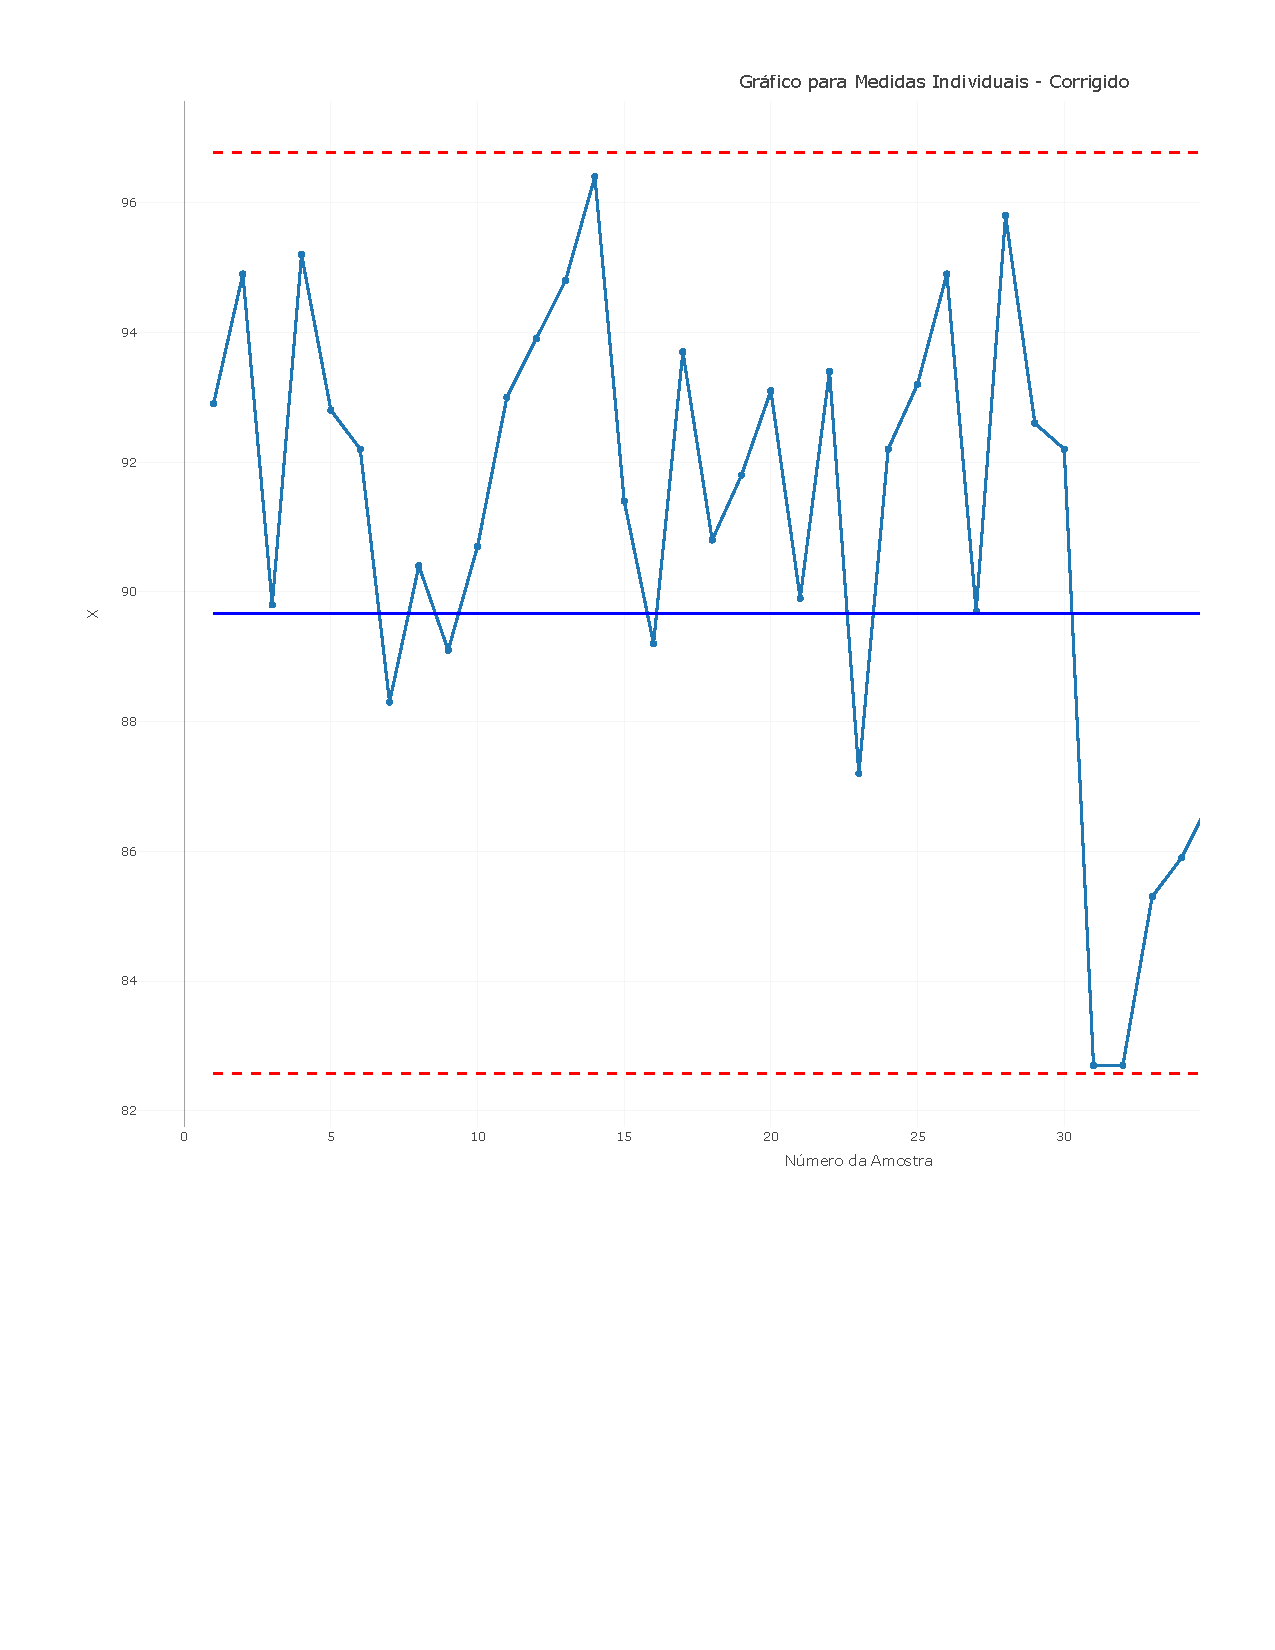
\includegraphics[keepaspectratio]{Controle_de_qualidade--3-_files/figure-pdf/unnamed-chunk-25-1.pdf}}

\subsubsection{Conclusão}\label{conclusuxe3o}

\subsubsection{\texorpdfstring{O gráfico de \(X\) e \(\bar{AM}\) é usado
no controle estatístico de processos com amostras individuais, sendo
fácil de implementar e eficaz para monitorar a média e a variabilidade
ao longo do
tempo.}{O gráfico de X e \textbackslash bar\{AM\} é usado no controle estatístico de processos com amostras individuais, sendo fácil de implementar e eficaz para monitorar a média e a variabilidade ao longo do tempo.}}\label{o-gruxe1fico-de-x-e-baram-uxe9-usado-no-controle-estatuxedstico-de-processos-com-amostras-individuais-sendo-fuxe1cil-de-implementar-e-eficaz-para-monitorar-a-muxe9dia-e-a-variabilidade-ao-longo-do-tempo.}

\subsubsection{Suas limitações incluem menor sensibilidade a pequenas
variações, susceptibilidade a valores atípicos e incapacidade de
identificar causas de variação, exigindo análises
complementares.}\label{suas-limitauxe7uxf5es-incluem-menor-sensibilidade-a-pequenas-variauxe7uxf5es-susceptibilidade-a-valores-atuxedpicos-e-incapacidade-de-identificar-causas-de-variauxe7uxe3o-exigindo-anuxe1lises-complementares.}

\subsubsection{Apesar dessas limitações, é uma ferramenta útil para
detectar mudanças em processos individuais, especialmente quando
combinada com outras técnicas
estatísticas.}\label{apesar-dessas-limitauxe7uxf5es-uxe9-uma-ferramenta-uxfatil-para-detectar-mudanuxe7as-em-processos-individuais-especialmente-quando-combinada-com-outras-tuxe9cnicas-estatuxedsticas.}




\end{document}
